\documentclass[conference]{IEEEtran}
%% SECON 2013 addition:
\makeatletter
\def\ps@headings{%
\def\@oddhead{\mbox{}\scriptsize\rightmark \hfil \thepage}%
\def\@evenhead{\scriptsize\thepage \hfil \leftmark\mbox{}}%
\def\@oddfoot{}%
\def\@evenfoot{}}
\makeatother
\pagestyle{headings} 

\ifCLASSINFOpdf
  % \usepackage[pdftex]{graphicx}
  % declare the path(s) where your graphic files are
  % \graphicspath{{../pdf/}{../jpeg/}}
  % and their extensions so you won't have to specify these with
  % every instance of \includegraphics
  % \DeclareGraphicsExtensions{.pdf,.jpeg,.png}
\else
  % or other class option (dvipsone, dvipdf, if not using dvips). graphicx
  % will default to the driver specified in the system graphics.cfg if no
  % driver is specified.
  % \usepackage[dvips]{graphicx}
  % declare the path(s) where your graphic files are
  % \graphicspath{{../eps/}}
  % and their extensions so you won't have to specify these with
  % every instance of \includegraphics
  % \DeclareGraphicsExtensions{.eps}
\fi
% *** MATH PACKAGES ***
%
\usepackage[cmex10]{amsmath}
\usepackage{amsfonts}
\usepackage{graphicx, epsfig}
\usepackage{color}
\usepackage{subfigure}
\usepackage{xspace}
\usepackage{algorithm}
\usepackage{algpseudocode}
\usepackage{breqn}
\usepackage{cite}

\renewcommand{\thealgorithm}{}
\algnewcommand{\LineComment}[1]{\State \(\triangleright\) #1}
% A popular package from the American Mathematical Society that provides
% many useful and powerful commands for dealing with mathematics. If using
% it, be sure to load this package with the cmex10 option to ensure that
% only type 1 fonts will utilized at all point sizes. Without this option,
% it is possible that some math symbols, particularly those within
% footnotes, will be rendered in bitmap form which will result in a
% document that can not be IEEE Xplore compliant!
%
%\usepackage{array}
%\usepackage{mdwmath}
%\usepackage{mdwtab}
%\usepackage{eqparbox}
%\usepackage[tight,footnotesize]{subfigure}
%\usepackage[caption=false]{caption}
%\usepackage[font=footnotesize]{subfig}
%\usepackage[caption=false,font=footnotesize]{subfig}
%
%\usepackage{fixltx2e}

%\usepackage{stfloats}

%\usepackage{url}

% correct bad hyphenation here
\hyphenation{net-works}

\DeclareMathOperator*{\E}{\mathbb{E}}
\DeclareMathOperator*{\argmax}{arg\,max}

\begin{document}
%
% paper title
% can use linebreaks \\ within to get better formatting as desired
\title{Stochastic Formulation of Scalability and Quality-of-Information Satisfiability in Wireless Networks}

\IEEEoverridecommandlockouts

% author names and affiliations
% use a multiple column layout for up to three different
% affiliations

%\author{\IEEEauthorblockN{Scott Rager}
%\IEEEauthorblockA{Department of Computer Science and Engineering\\
%Pennsylvania State University\\
%University Park, PA 16802\\
%Email: rager@psu.edu}}

%\author{\IEEEauthorblockN{Scott Rager, Ertugrul Ciftcioglu, Thomas La Porta}
%\IEEEauthorblockA{Department of Computer Science\\
%and Engineering\\
%Pennsylvania State University\\
%University Park, PA 16802\\
%Email: rager@psu.edu, enc118@psu.edu, tlp@cse.psu.edu}
%\and
%\IEEEauthorblockN{Alice Leung, William Dron}
%\IEEEauthorblockA{Raytheon BBN Technologies\\
%Cambridge, MA 02138\\
%Email: aleung@bbn.com, wdron@bbn.com}
%\thanks{Research was sponsored by the U.S. Army Research Laboratory under the Network Science Collaborative Technology Alliance, Agreement Number W911NF-09-2-0053.} 
%}

%\author{
%  \IEEEauthorblockN{Scott T. Rager\IEEEauthorrefmark{1} \quad Ertugrul N. Ciftcioglu\IEEEauthorrefmark{2}  \quad Ram Ramanathan\IEEEauthorrefmark{3} \quad Thomas F. La Porta\IEEEauthorrefmark{1} \quad Ramesh Govindan\IEEEauthorrefmark{4} \\
%  }
%  \IEEEauthorblockA{
%  	\IEEEauthorrefmark{1}The Pennsylvania State University, University Park, PA 16802\\
%	\IEEEauthorrefmark{2}IBM Research, Yorktown Heights, NY 10598 \\
%  \IEEEauthorrefmark{3}Raytheon BBN Technologies, Cambridge, MA 02138 \\
%  \IEEEauthorrefmark{4}University of Southern California, Los Angeles, CA 90089
%  }
%
%  Email:  rager@psu.edu, enciftci@us.ibm.com , ramanath@bbn.com, tlp@cse.psu.edu, ramesh@usc.edu
%\thanks{Research was sponsored by the U.S. Army Research Laboratory under the Network Science Collaborative Technology Alliance, Agreement Number W911NF-09-2-0053.} 
%}


% for over three affiliations, or if they all won't fit within the width
% of the page, use this alternative format:
% 
%\author{\IEEEauthorblockN{Michael Shell\IEEEauthorrefmark{1},
%Homer Simpson\IEEEauthorrefmark{2},
%James Kirk\IEEEauthorrefmark{3}, 
%Montgomery Scott\IEEEauthorrefmark{3} and
%Eldon Tyrell\IEEEauthorrefmark{4}}
%\IEEEauthorblockA{\IEEEauthorrefmark{1}School of Electrical and Computer Engineering\\
%Georgia Institute of Technology,
%Atlanta, Georgia 30332--0250\\ Email: see http://www.michaelshell.org/contact.html}
%\IEEEauthorblockA{\IEEEauthorrefmark{2}Twentieth Century Fox, Springfield, USA\\
%Email: homer@thesimpsons.com}
%\IEEEauthorblockA{\IEEEauthorrefmark{3}Starfleet Academy, San Francisco, California 96678-2391\\
%Telephone: (800) 555--1212, Fax: (888) 555--1212}
%\IEEEauthorblockA{\IEEEauthorrefmark{4}Tyrell Inc., 123 Replicant Street, Los Angeles, California 90210--4321}}




% use for special paper notices
%\IEEEspecialpapernotice{(Invited Paper)}




% make the title area
\maketitle


\begin{abstract}
\boldmath
%area
%problem
%solution
%methodology
%results
%takeaway
This is where the abstract will be....essentially we're extending the ideas in the conference submission to include probabilistic requirements.

\end{abstract}

% IEEEtran.cls defaults to using nonbold math in the Abstract.
% This preserves the distinction between vectors and scalars. However,
% if the conference you are submitting to favors bold math in the abstract,
% then you can use LaTeX's standard command \boldmath at the very start
% of the abstract to achieve this. Many IEEE journals/conferences frown on
% math in the abstract anyway.

% no keywords




% For peer review papers, you can put extra information on the cover
% page as needed:
% \ifCLASSOPTIONpeerreview
% \begin{center} \bfseries EDICS Category: 3-BBND \end{center}
% \fi
%
% For peerreview papers, this IEEEtran command inserts a page break and
% creates the second title. It will be ignored for other modes.
\IEEEpeerreviewmaketitle


%\section{Introduction}
\label{sec:intro}

% we use QoI
% we are modeling which is easier than experimentation
% we are looking at scalability, not optimizing networks

%area
%problem
Traditional approaches to studying network scalability and performance limitations have been focused on finding theoretical limits on throughput and delay.  In many applications, however, the relationship between these metrics and the effectiveness of the network is highly non-linear.  Therefore, having a framework to evaluate network scalability with respect to achievable \emph{Quality of Information} (QoI) requirements is necessary.

Additionally, while theoretical, asymptotic analysis of individual network topologies, protocols, etc. is important, such analysis lacks the ability to quickly obtain an accurate estimate of a projected network's abilities when these individual components are pieced together.  Often, extensive simulation or experimentation testbeds must be created to test proposed network setups, which is difficult and time-consuming.  

As an example, imagine being given the task of deploying a wireless sensor network for a particular application.  Given a proposed network with a defined size, topology, parameters, and protocols, what is the level of QoI requirements it can support?  Now, consider the converse:  Given a certain QoI that is desired by users of a network, what is the maximum number of nodes that the network can support?  Which has a bigger impact on this scalability, the imposed information requirements, or the strict timeliness requirements?

Our main contribution in this paper is a novel framework that can predict scalability and performance of a network with respect to QoI requirements for answering such questions.  We explain this framework in detail in Section \ref{sec:qoi_scalability} and provide example applications in Section \ref{sec:example_applications}.  As a second contribution we extend this framework in Section \ref{sec:delay_char}, capturing the stochastic nature of query sources and destinations as well as data requirements, and show that it can be used to characterize query delays.  In both cases, we provide results from realistic implementations in the ns-3 network simulation environment.  

We also present several pieces of supporting work.  First we provide an example of an application that relies on QoI to highlight the difference in QoI and traditional metrics in Section \ref{sec:qoi_model}.  We show in Section \ref{sec:network_design} that our framework is also quite useful in quickly and easily understanding the impact of parameters and design choices, providing a secondary benefit to network designers of allowing them to compare networks and identify tradeoffs.  Finally, we show how the framework can also provide bounds on QoI capacity in some applications in Section \ref{sec:scal_feasible_qoi}.

%in contrast to discovering theoretical, asymptotic limits, a need for network designers is to quickly obtain an accurate estimate of a network's abilities.  The goal of this paper is not in optimizing network performance; instead, we show in Section \ref{sec:network_design} that this model can also be used to quickly and easily understand the impact of parameters and design choices.  This ability provides a secondary benefit to network designers of allowing them to compare networks and identify tradeoffs. 

% this assumption is unrealistic for many applications. For these reasons, we adopt \emph{Quality of Information} (QoI), which can include a number of information attributes (many of which are context-dependent), such as completeness, diversity, credibility, creation time, and timeliness, as our measure of network performance.  Specifically, in this work, we focus on satisfiability of completeness and timeliness, explained in detail in Section \ref{sec:qoi_model}.

%The second contribution differentiating this work from previous analysis is that we focus on providing a framework that can be adjusted to determine scalability and QoI satisfiability for any instance of a network.  The wide applicability and easy reuse of this framework make it easy to compare protocols, topologies, traffic models, etc., without creating extensive simulation or experimentation testbeds, which is a much more difficult task.

%Finally, in contrast to discovering theoretical, asymptotic limits, this framework seeks to quickly obtain an accurate estimate of a network's abilities.  The goal of this paper is not in optimizing network performance; instead, we show in Section \ref{sec:network_design} that this model can also be used to quickly and easily understand the impact of parameters and design choices.  This ability provides a secondary benefit to network designers of allowing them to compare networks and identify tradeoffs. 

%why not solved
%Currently, no framework exists that provides a methodology to predict scalability and performance with respect to QoI requirements.  In this paper, our contribution is to provide such a framework.%, which we do in Section \ref{sec:qoi_scalability}.  In Section \ref{sec:validation}, we prove its effectiveness by comparing it to simulations performed in the ns3 network simulation package.  We provide examples of how it is also useful in network design in Section \ref{sec:network_design}.  Finally, we also take the concept one step further in Section \ref{sec:scal_feasible_qoi} with the introduction of a \emph{scalably feasible QoI region}, which describes the maximum QoI capacity of a particular network scenario.

%insight
%contribution
%Using timely, similarity-based image collection as a motivating application, we show the application of our framework in determining realistic limitations of an actual network scenario and validate their accuracy with simulations results from testing performed with the ns3 network simulation package.  Then, we explore the impact of changing network parameters, like topology, network size, bandwidth, etc. on satisfiable QoI and scalability, answering the questions of the impact of design choices explored above.  Finally, we also take the concept one step further with the introduction of a \emph{scalably feasible QoI region}, which describes the maximum QoI capacity of a particular network scenario. 

%Imagine given the task of deploying an ad hoc network for a particular task or application.  In executing this task, it is important to first recognize the correct metrics by which the network's performance is properly measured.  Specifically, in these networks, traditional metrics of throughput, latency, jitter, etc. are no longer the only focus.  Furthermore, the implicit assumption that linear improvements in these metrics provide an equivalently linear increase in utility to users of the network is unrealistic, because the usefulness of data is highly dependent on context.  For that reason, we instead use \emph{Quality of Information} (QoI), which includes a number of data attributes  (many of which are context-dependent), such as completeness, information diversity, credibility, creation time, and timeliness, as a general measure of network performance.  
%In addition to understanding how to properly measure the network performance, effective design of an ad hoc network requires understanding the QoI and scalability limitations of a proposed deployment.  For example, we may want to answer questions like:  With a set of traffic requirements, what is the maximum number of nodes the network can support?  Or, alternatively, given a proposed network description, how much data can we support, and what is the QoI of that data?  Furthermore, the impact of design choices on these limitations is even more valuable in optimal design.  Here, we propose answers to questions like the following:  How sensitive is delay to network size for a given topology?  Or, How does increasing requirements for completeness of information affect network size when we have a strict timeliness requirement?

%\section{Related Work}
\label{sec:related_work}

The scalability model derived in this work is inspired by the symptotic scalability framework outlined in \cite{symptotics_journal}, which has been previously applied to content-agnostic static networks \cite{symptotics_framework_scalability} and mobile networks \cite{scal_analysis_mobility}. {\color{blue}We provide several differences and additional analysis here compared to these works, which mainly stem from our use of QoI requirements instead of static data rates. The first difference is that we are able to evaluate performance and scalability under timeliness constraints, which is not possible under any of these prior works. Second, we illustrate the effects on an application's performance, which is not linear with respect to data rates in most cases. Additionally, we provide a formulation that includes parameters characterized by random variables. This improved modeling allows us to characterize expected delays with a probability distribution, which the previous works do not provide.}

Other works characterize the capacity of wireless networks, like \cite{li_capacity, gupta2000capacity}, but all do so by considering how networks scale asymptotically or by analyzing specific network instances instead of developing a general model. {\color{blue}Experimental techniques, like Response Surface Methodology \cite{khuri2010response}, discrete-event simulators \cite{ns3}, and real wireless network testbeds \cite{iot_lab_exp_platform, wsn_testbed, wisebed} may be applied to solve the problem we do, and, in fact, after finalizing a network design, implementing one of these methods to further verify capabilities is desirable. The anticipated applications of this work, however, are different in that either there is not enough time to develop a realistic simulation or implementation, or the goal is to evaluate a number of combinations of design choices, such that implementing each possible combination and/or running trials over the sets of independent parameters would be too time-intensive.}

A large number of works provide definitions for QoI and frameworks that utilize it.  We will address only the most relevant ones here.  Primarily, QoI has been considered from a number of angles including routing \cite{quality_aware_routing_tan}, scheduling/rate control \cite{toward_qoi_rate_control,explor_vs_exploit}, and impact on usage of network resources \cite{qoi_aware_mobile_apps}. Our focus is on a broader scale here, though, modeling scalability and limitations of an entire network.  

%The work in \cite{qoi_aware_mobile_apps} evaluates the impact of varying QoI requirements on usage of network resources, which is certainly related to this paper.  Our focus is on a broader scale than this work, though, by modeling an entire network instead of a single node as the authors do in \cite{qoi_aware_mobile_apps}.

A framework called Operational Information Content Capacity (OICC) is outlined in \cite{oicc_journal}, which describes the obtainable region of QoI, a notion similar to the \emph{scalably feasible QoI region} developed here. OICC differs, though, in the fact that it does not provide any method for determining the possible size of the network or impact of network design choices like medium access protocols. We also note that a notion similar to QoI satisfiablility was considered in \cite{qoi_outage} which addresses resource allocation for long-term average QoI outage satisfaction. However, the focus of \cite{qoi_outage} is energy-efficient scheduling and power allocation in a single-hop three-node network rather than scalability. 

In Section \ref{sec:qoi_model}, we use similarity-based image collection as an example of an application that is best evaluated using QoI.  This application has previously been considered in \cite{photonet} and \cite{mediascope}. Our scope is greater than that of \cite{photonet}, which does not consider attributes of timeliness, nor the consideration of transmission rates and network topology.  We use the same similiary-based image selection algorithm as in \cite{mediascope}, but provide new methods of quantifying QoI.% considers a smartphone application where different queries called Top-K, Spanner, and K-means Clustering are defined.  We use these same similarity-based image selection algorithms, but we provide new methods of quantifying QoI from them.

\begin{figure*}[t!]
\centering
    \subfigure[Top-K: Sum Similarity]{
        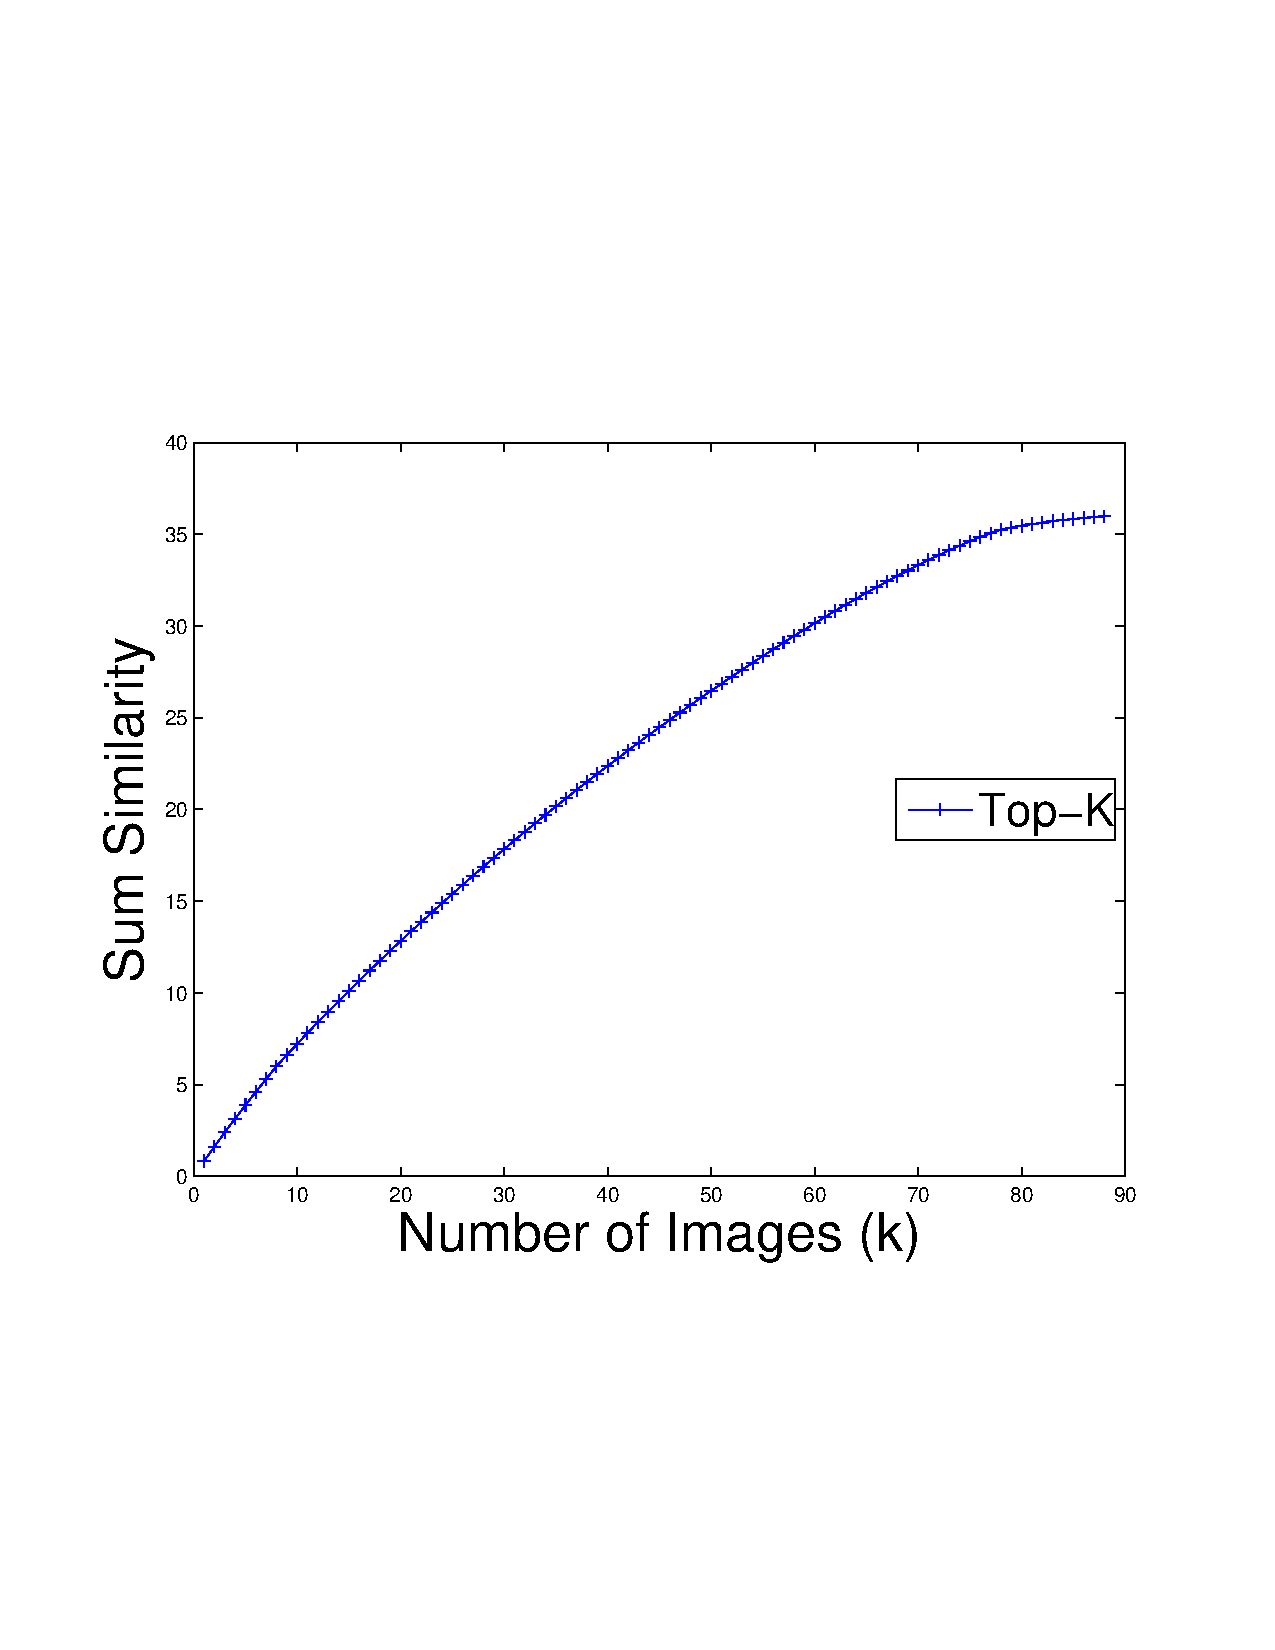
\includegraphics[clip=true, trim = 17mm 65mm 25mm 70mm, scale=0.23]{figures/topk/topk_sum_sim_color.pdf}
        \label{fig:topkSumSim}
        }
    \subfigure[Top-K: Avg. Match Target]{
        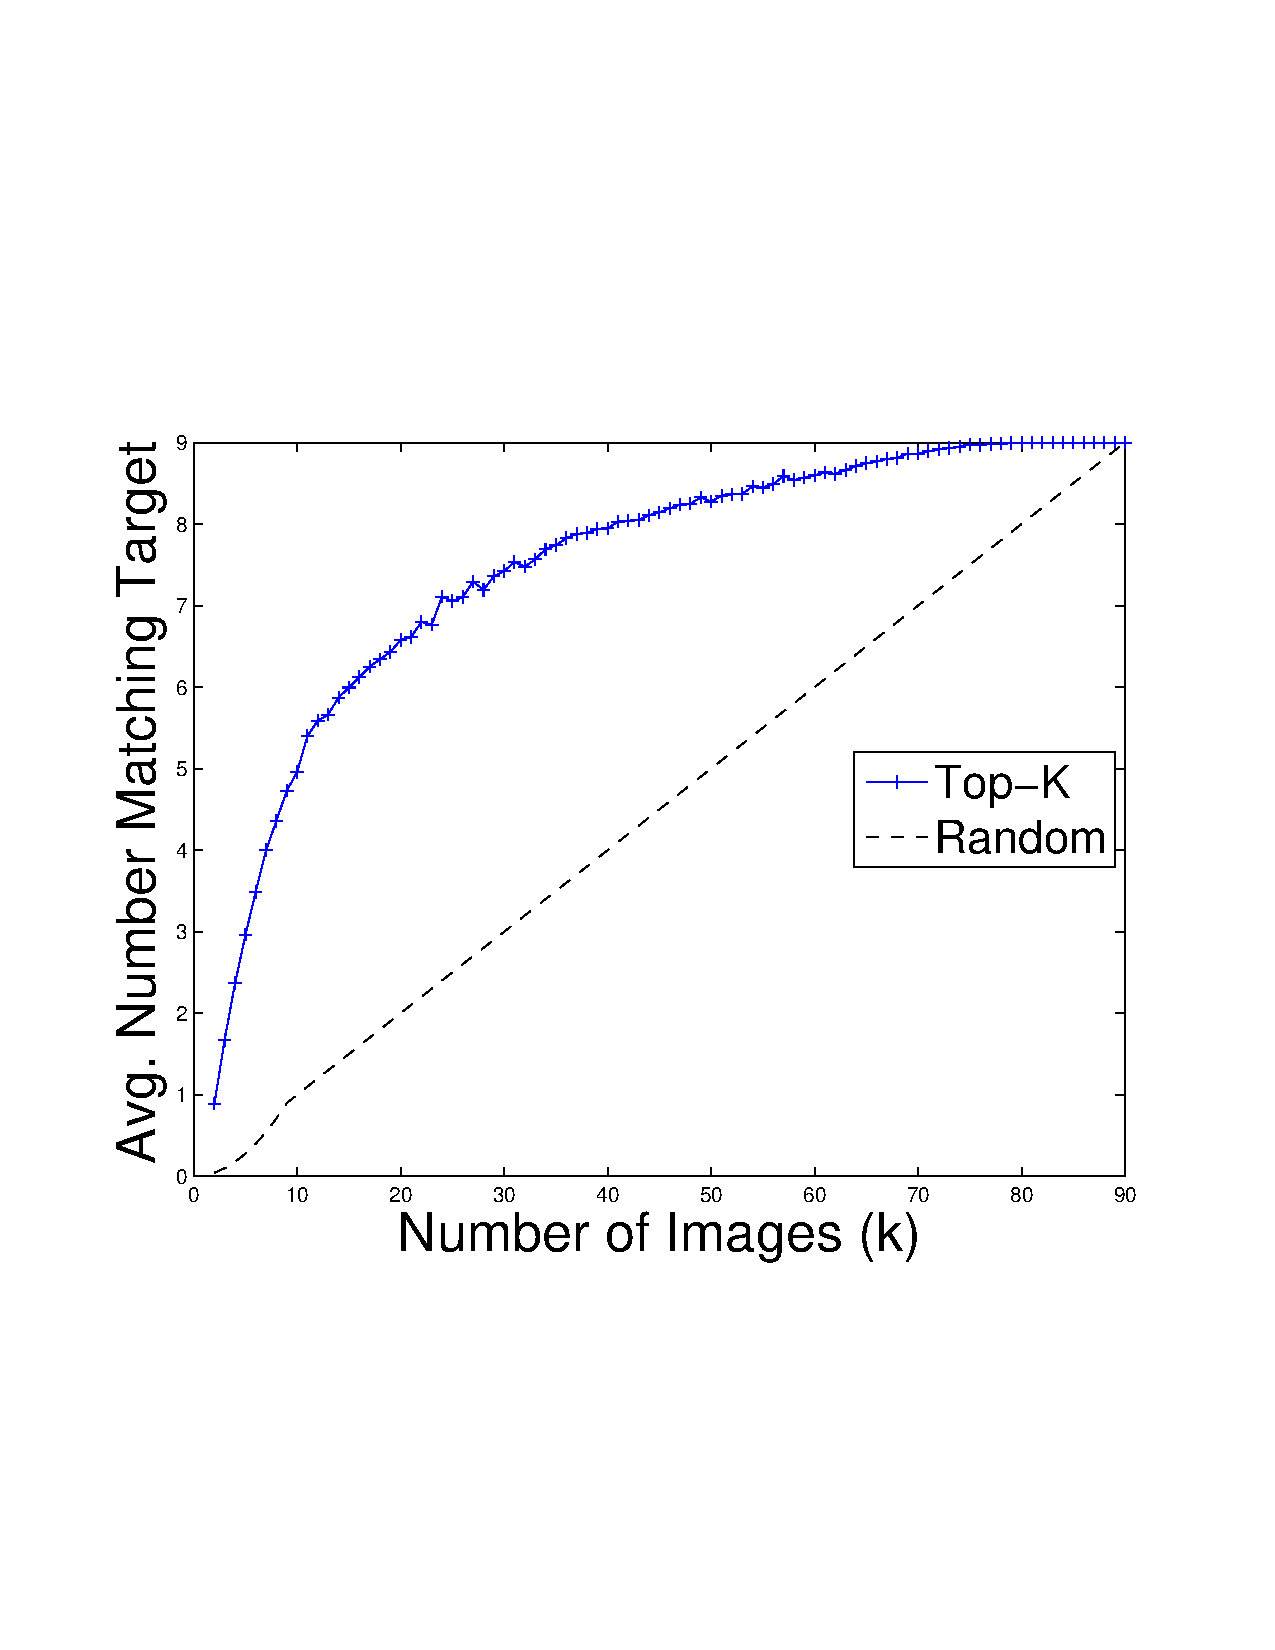
\includegraphics[clip=true, trim = 17mm 65mm 25mm 70mm, scale=0.23]{figures/topk/avg_num_matching_color.pdf}
        \label{fig:topkAvgNumSameSet}
        }
    \subfigure[Spanner: Sum Dissimilarity]{
        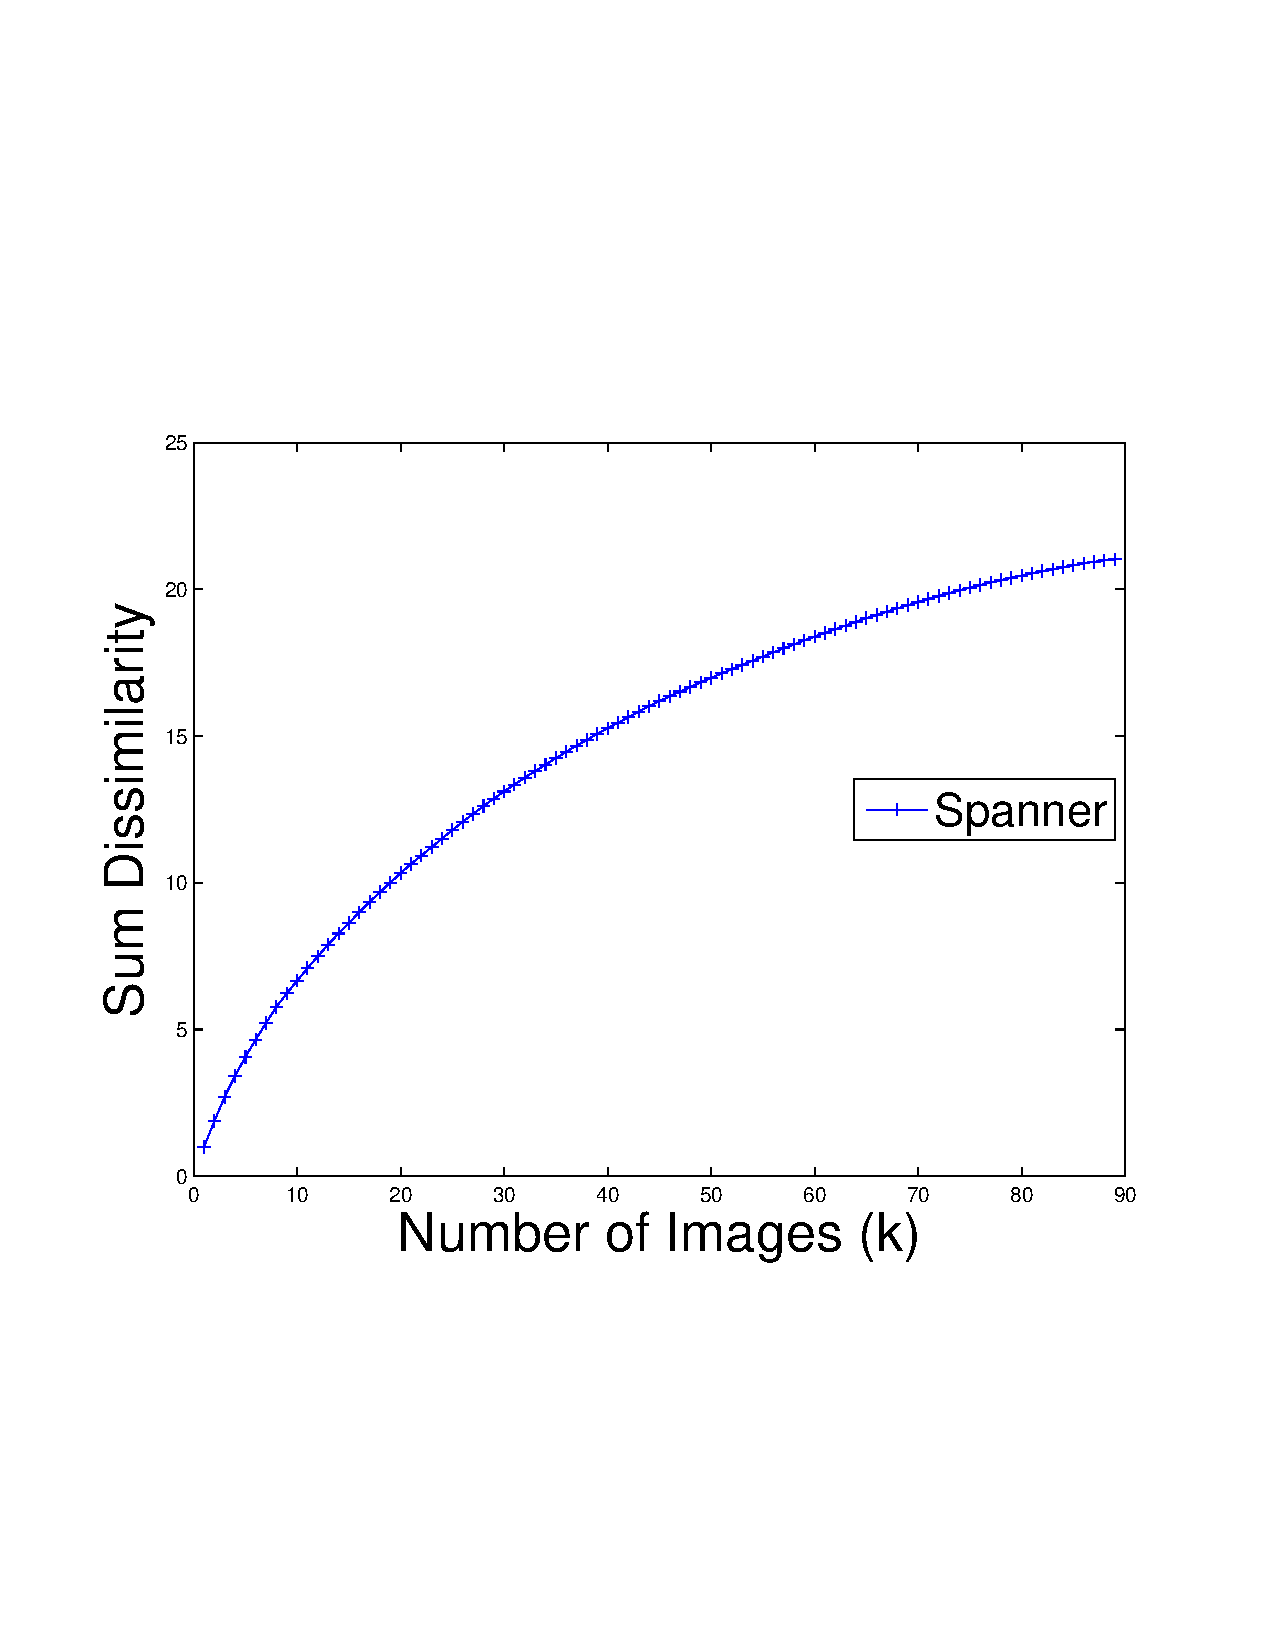
\includegraphics[clip=true, trim = 17mm 65mm 25mm 70mm, scale=0.23]{figures/spanner/spannerCumulativeDist_color.pdf}
        \label{fig:spanSumDissim}
        }
    \subfigure[Clustering: Cover All Sets]{
        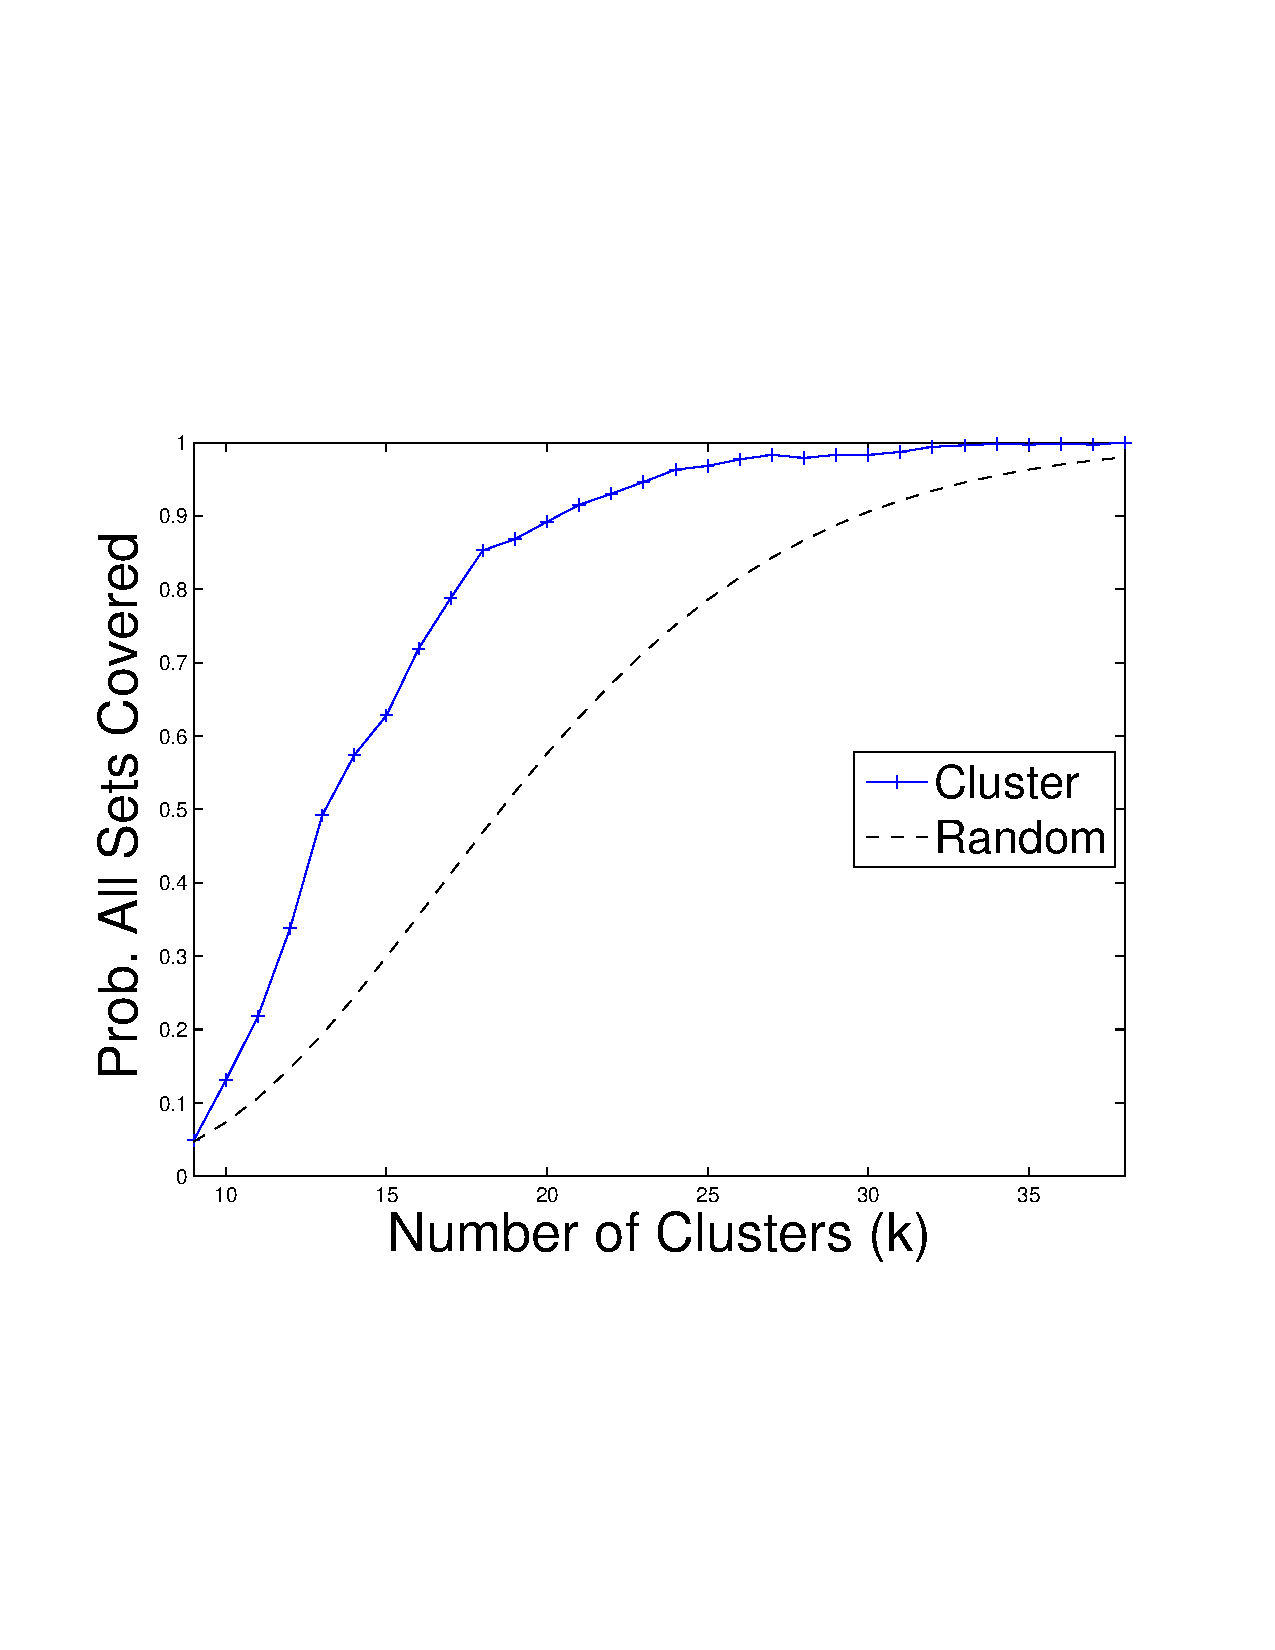
\includegraphics[clip=true, trim = 16mm 65mm 25mm 70mm, scale=0.23]{figures/cluster/perc_all_sets_covered_vary_k_color.pdf}
        \label{fig:clusterAvgNumSetsCov}
        }        
   \caption{Completeness metrics for the three image selection algorithms. Each exhibits a diminishing return as more images are added.}
   \label{fig:completeness_exp_results}
   \vspace{-4mm}
\end{figure*}

\section{QoI Model}
\label{sec:qoi_model}

Let us define the following terms:

\begin{itemize}
  \item $W$ = Channel Rate (bits/second)
  \item $T$ = Timeliness Requirement (seconds)
  \item $k_{req}$ = Number of required images
  \item $I_S$ = Size of each image (bits)
  \item $CF$ = Channel Factor
  \item $TF$ = Traffic Factor
  \item $P_S$ = Packet size
  \item $DF$ = Delay Factor
  \item $PL$ = Path Length
  \item $p_{i,j}$ = Probability of a flow from $i$ to $j$
\end{itemize}

In the conference submission we derived the following equation for scalability that uses each of these defined terms:
\begin{equation}
	W \cdot T - k_{req} \cdot I_S \cdot CF \cdot TF - P_S \cdot DF \cdot (PL-1) \geq 0	
\end{equation}

If we rearrange this equation, we can view the satisfiability of timeliness in terms of delay components:
\begin{equation}
	T \geq \frac{ k_{req} \cdot I_S \cdot CF \cdot TF}{W} + \frac{P_S \cdot DF \cdot (PL-1)}{W}
\end{equation}

In our previous analysis, we strive to determine the limits of this timeliness satisfiability by utilizing some static values and some average values where appropriate in this relation.  The resulting analysis provided approximate values for QoI satisfiability and network scalability, but what if we want to expand satisfiability to a stochastic definition?  And/or can we provide more accurate estimations by using more detailed models of the actual values of the parameters in the above list? 

To begin answering these questions, we can look at some of these parameters in more detail and use more accurate descriptions of them by classifying them as Random Variables with appropriate probability density distributions.  In this case, we start by examining a line network.  Its simple structure and routing make it a nice, simple topology to use as an exploratory model.  Here, the same traffic model as in the conference submission is also used.  In this model, each node is a source of a query that is delivered to a randomly chosen destination.  

\subsection{Traffic Factor}

Let $\rho(x)$ be the number of shortest paths of all other nodes that include node $x$ (NOTE: Is this the same as Betweeness Centrality?).  Let $F_{ij}$ be represent the existence of a flow existing from node $i$ to node $j$.  We assume that $F_{ij}$ is equal to $1$ with probability $p_f$ and $0$ otherwise.  Then, the traffic factor of a node $x$, $R_x$, is given by the sum of $F_{ij}$ for all $\rho(x)$ pairs $(i,j)$ in which $x$ is along the shortest path.  Assuming that $F_{ij}$ is i.i.d. for all pairs $(i,j)$, then $R_x$ can be approximated by a Normal RV with mean $\rho(x) p_f$ and variance $\rho(x) p_f (1-p_f)$:

\begin{equation}
	f_{R_x} = \mathcal{N}(\rho(x) p_f, \rho(x) p_f (1-p_f)) 
\end{equation}

Let's consider a flow originating at node $i$, and call the destination of the flow $j$.  When characterizing the largest contributor to delay, we need to determine the maximum expected Traffic Factor through which the flow will be forwarded.  We will use $TF_{i}$ to represent that maximum expected Traffic Factor for a flow with origin $i$.  To get a distribution for overall delay, we want to derive a distribution for this value.  We will use $P_{TF_i}$ to represent the PDF of the Traffic Factor for this flow originating at node $i$.  
We need to first find the node that has the largest expected TF between node $i$ and node $j$, so we need to find the node $x'$ that has the maximum expected TF.  Since $p_f$ is constant, the node with the maximum expected TF is:

\begin{equation}
\label{eq:max_tf_node}
	x' = \argmax_{x = [\min(i,j), \max(i,j)]} \rho(x) 
\end{equation}

Then, we can say that the distribution of the TF for this flow would be

\begin{equation}
	f_{TF_{i}}(tf) = \mathcal{N}(\rho(x') p_f, \rho(x') p_f (1-p_f))
	\label{eq:pdf_TF_1}
\end{equation}

Given a network graph, values of $\rho(x)$ and the solution of ($\ref{eq:max_tf_node}$) could be analytically determined for that specific case.  In networks with regular structure, though, we may be able to develop closed form expressions for 

\subsection{Path Length}

%\begin{figure}
%\begin{centering}
%    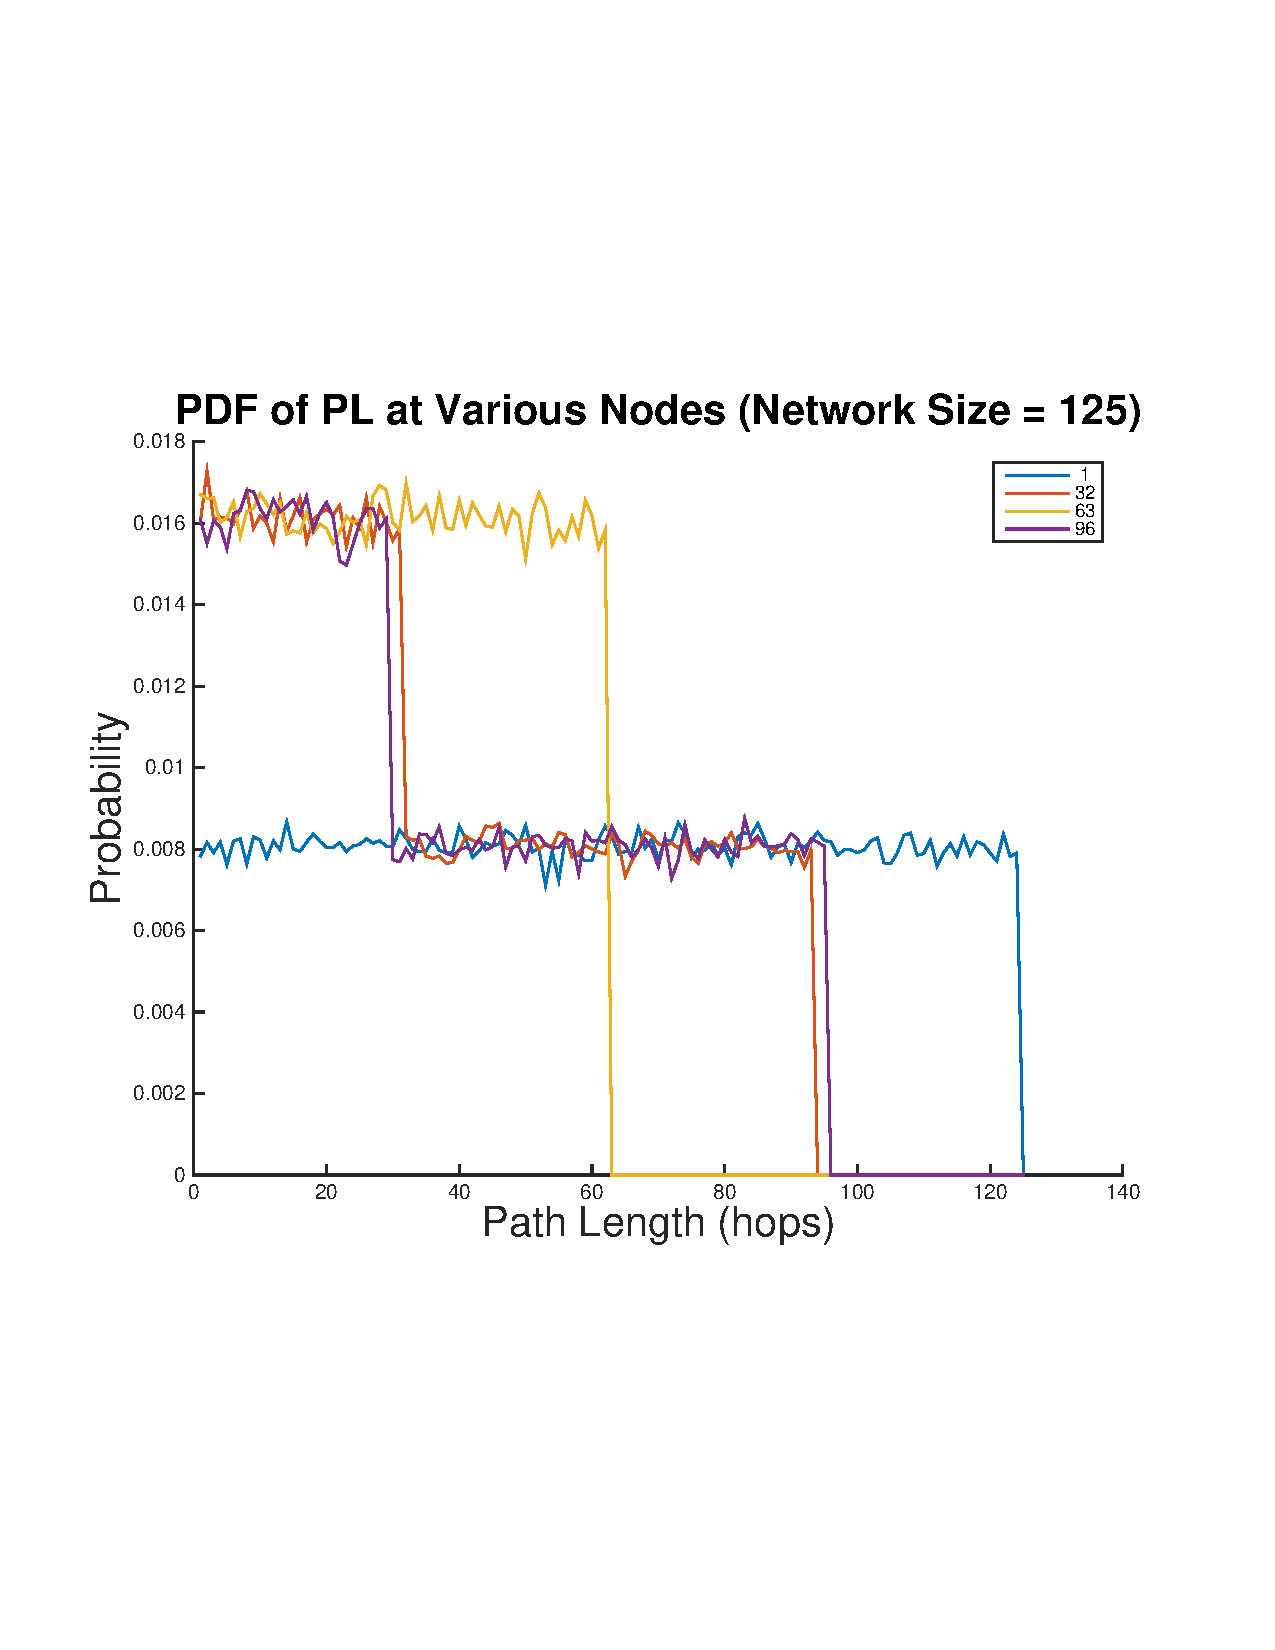
\includegraphics[scale=0.4, clip=true, trim=15mm 65mm 20mm 65mm]{figures/PL_PDFs_each_node_line_net_125.pdf}
%    \caption{Plotting the frequency of experienced Path Lengths for different node positions in a line network shows that PL can be modeled as disjoint Uniform Random Variables.}
%    \label{fig:PL_PDFs_line_net}
%\end{centering}
%\end{figure}
\begin{figure}
\begin{centering}
    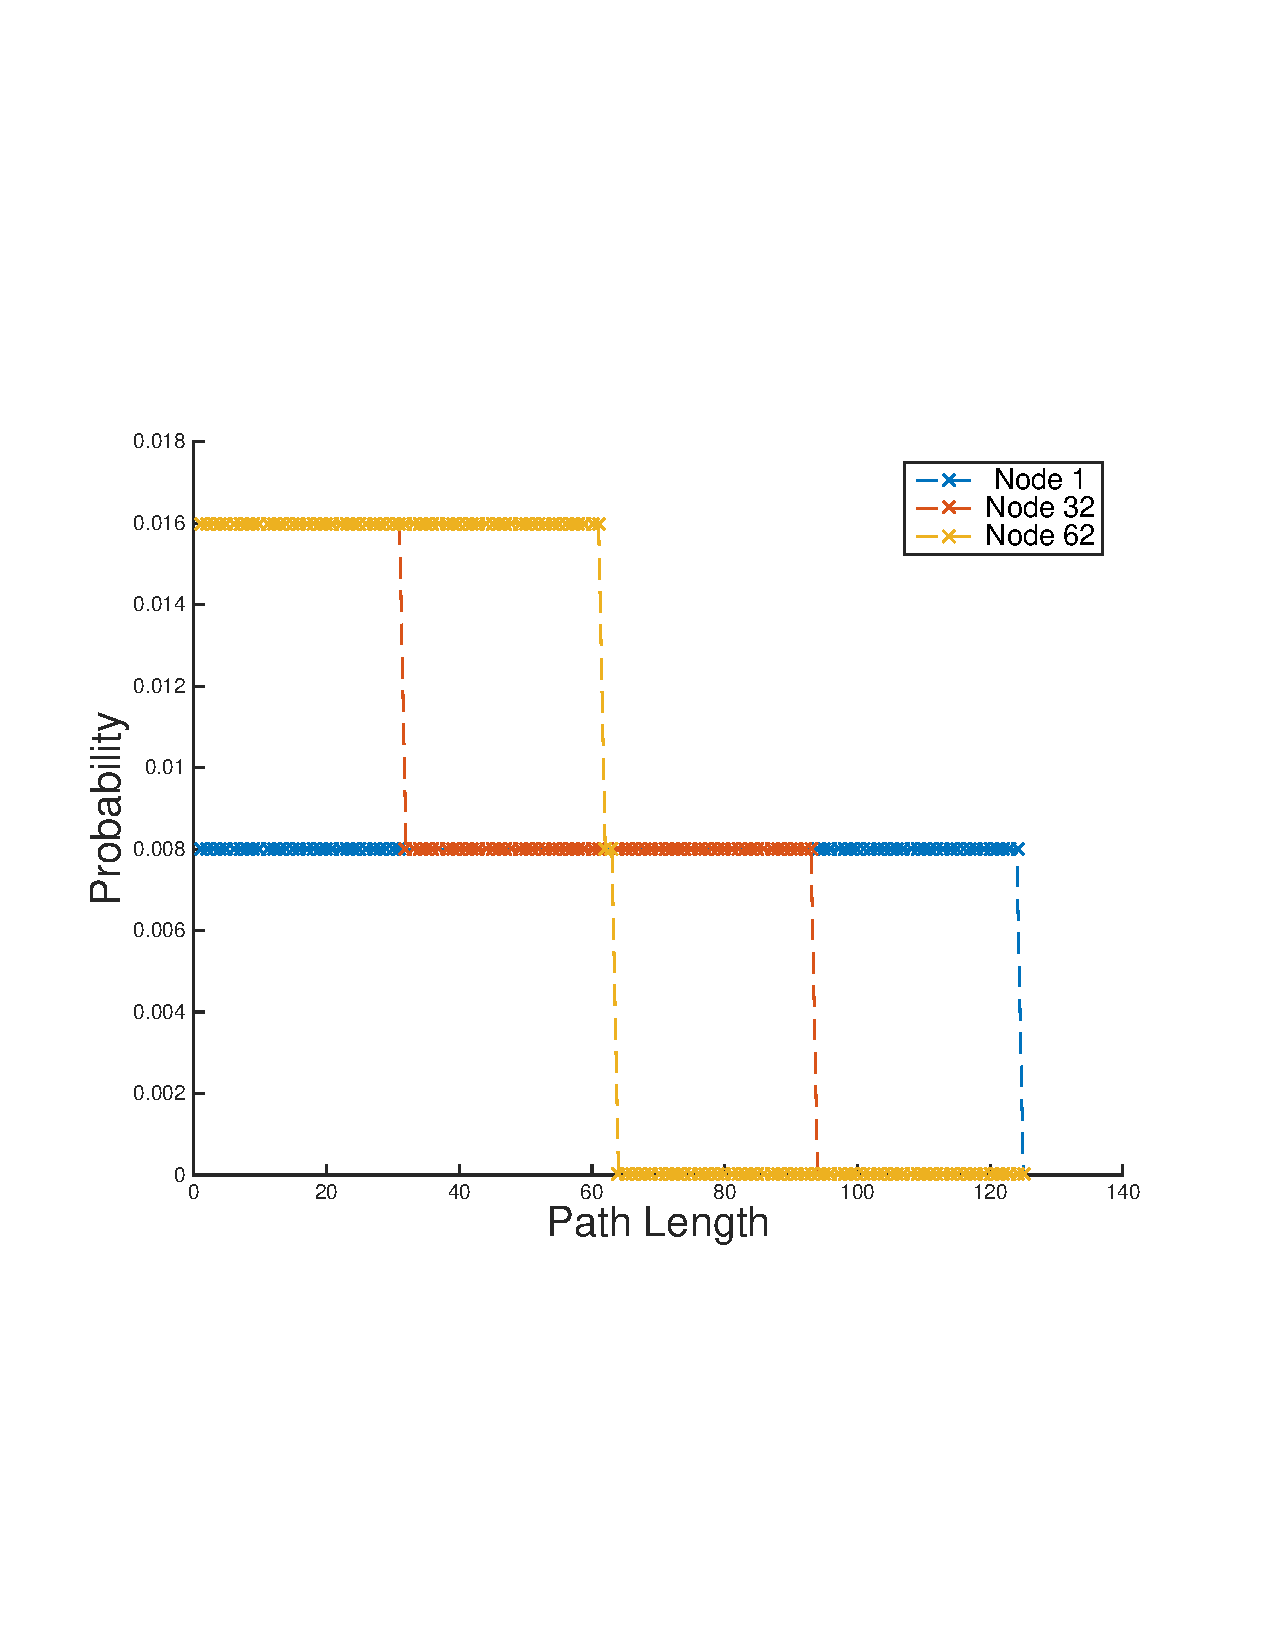
\includegraphics[scale=0.4, clip=true, trim=15mm 65mm 20mm 65mm]{figures/PDF_PL_line_net_125.pdf}
    \caption{PDF of Path Lengths for flows originating in edge cases of a line network.}
    \label{fig:PL_PDFs_line_net}
\end{centering}
\end{figure}

Next, we can capture the distribution of the path length given by flows originating in node $i$ of the network.  Once again, this distribution can be determined for any network given the topology with some simple computation, but we can provide expressions for some regular networks.


%Is the Delay Factor dependent on node position?  It must be...similar to path length, a node's position affects the probability of choosing a route with or against the flow of scheduling.  
%Finally, we can give a simple expression for the Delay Factor: 
%\begin{eqnarray*}
%	P_{DF_x}(l) &=&
%		\left\{\begin{array}{ll}
%		\frac{2}{N} & \mbox{for } 1 < l < \min(i,N-i) \\
%		\frac{1}{N} & \mbox{for } \min(i,N-i) \leq l \leq \max(i,N-i) \\
%		0 &\mbox{elsewhere}
%		\end{array}\right.
%\end{eqnarray*}




\section{Finding Bottleneck Flow}
\label{sec:bottleneck}

Again, we turn to the satisfiability equation, but use random variables for the Traffic Factor and Path Length, $TF_i$ and $PL_i$, respectively:
\begin{equation}
	T \geq \frac{ k_{req} \cdot I_S \cdot CF \cdot TF_i}{W} + \frac{P_S \cdot DF \cdot (PL_i-1)}{W}
\end{equation}
where we will call the total delay
\begin{equation}
	D_i = \frac{ k_{req} \cdot I_S \cdot CF \cdot TF_i}{W} + \frac{P_S \cdot DF \cdot (PL_i-1)}{W}
\end{equation}

Now, we want to identify which flow $i$, identified by its origin node, is most likely to be the flow that cannot be satisfied in the allotted timeliness.  To do so, we can simply find the value of $i$ that results in the largest $D_i$.

\begin{figure}
\begin{centering}
    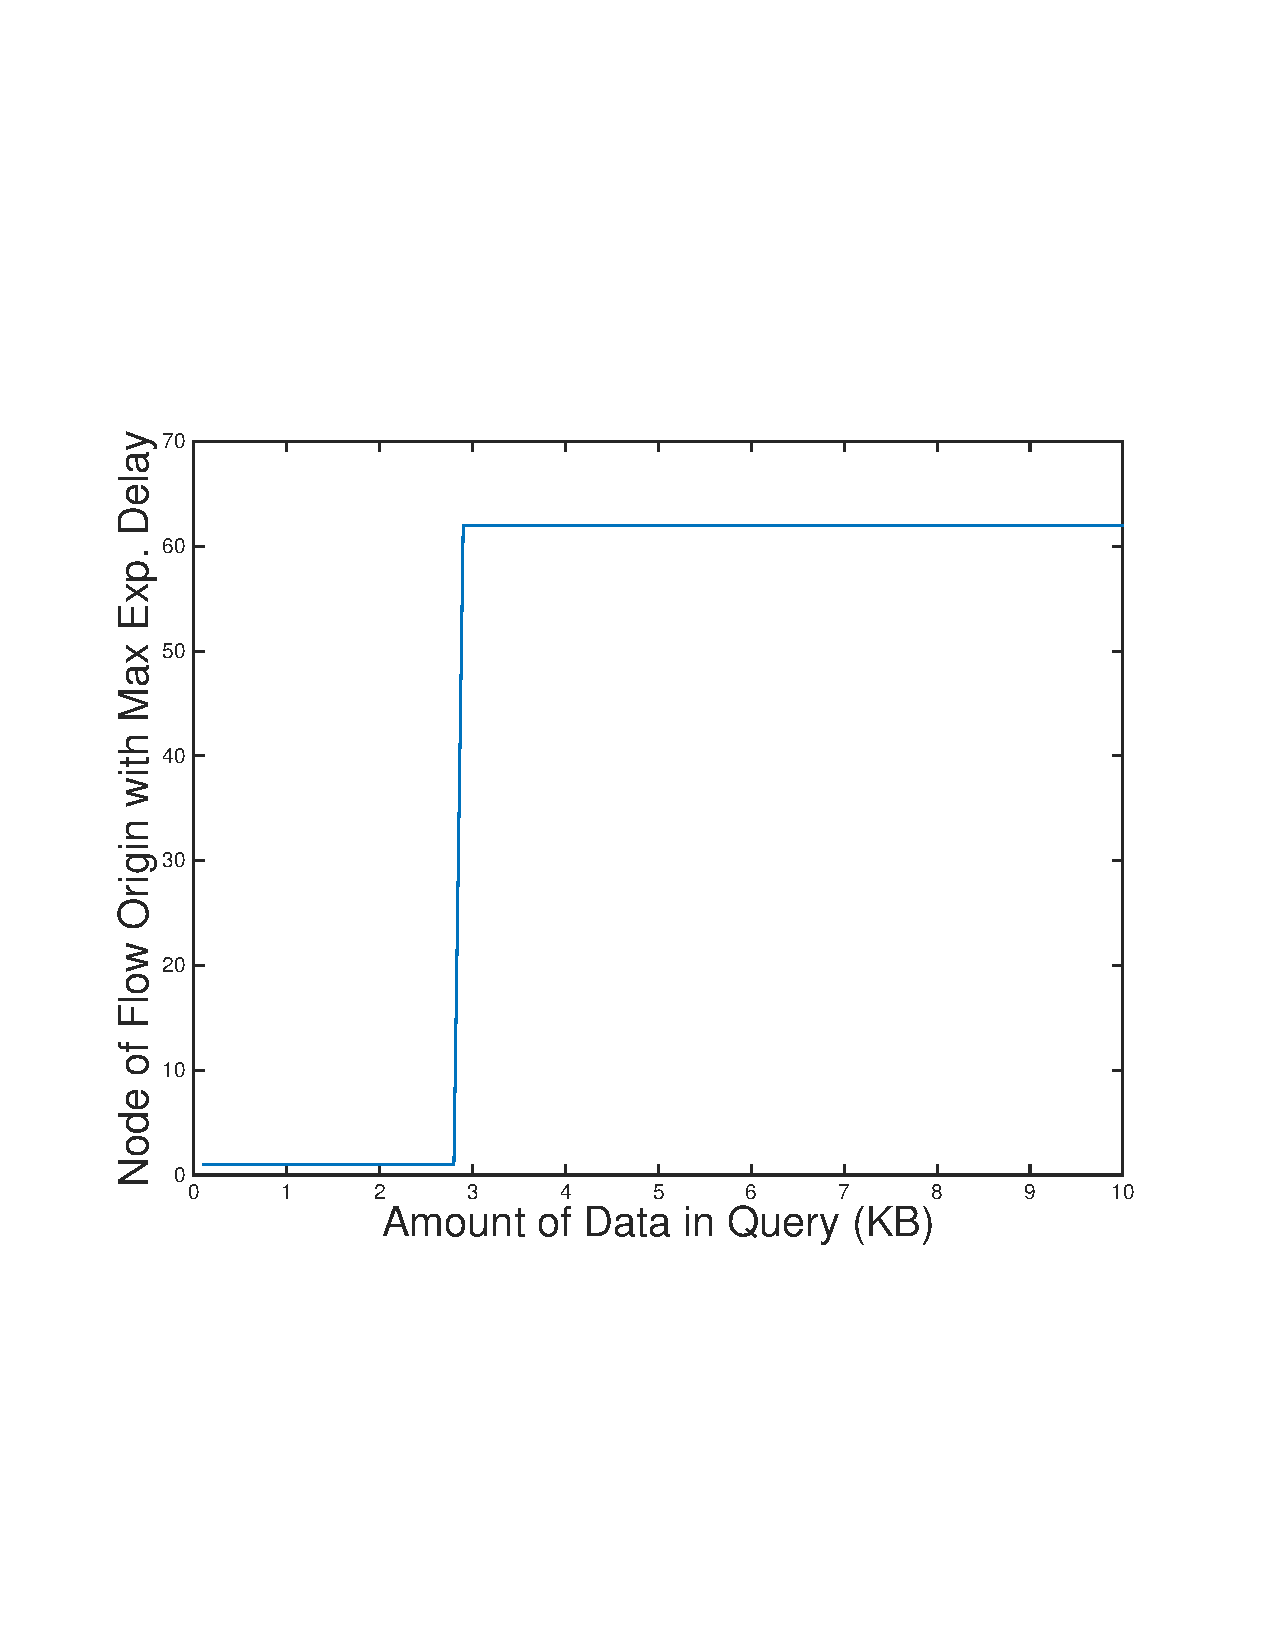
\includegraphics[scale=0.4, clip=true, trim=15mm 65mm 20mm 65mm]{figures/max_i_line_net_125.pdf}
    \caption{The value of $i$ (origin of a flow) that causes the maximum expected delay.}
    \label{fig:max_i_line_net}
\end{centering}
\end{figure}

Using the expected values for $TF_i$ and $PL_i$ from Figures \ref{fig:EV_TF_line_net} and \ref{fig:mean_PL_each_node_line_net}, we find the value of $i$ that maximizes $D_i$ for different data requirements, $B = k_{req}*I_S$.  Figure \ref{fig:max_i_line_net} shows that for low data requirements, the delay of multi-hop paths dominates, causing the ``Bottleneck" flow to be those that originate in node $1$ and have a larger expected path length.  At a point, though, as the amount of data required in the query grows, congestion will be the limiting factor in the network, making the Traffic Factor more important.  Thus, the node near the center of the network which will be likely to experience the highest amount of congestion become the source of flows with the highest delay.  In this case, we have $i = 62$, since the network has $125$ nodes (NOTE: It should probably be 63, but there is an ``off-by-one" error here because the definitions/formulations are not carefully derived to be correct on the boundaries).



\section{Probability of Satisfying Query}
\label{sec:prob_sat}

Now, we have an expression for delay that is built up using random variables for the values of $TF$ and $PL$.  The next useful formulation is providing an expression that describes the probability of a bottleneck flow satisfying its timeliness requirement considering the underlying distributions.  With this formulation, we can define scalability as a network in which the flow's probability of satisfiability exceeds some threshold $P_{thresh}$:
\begin{equation}
	P(D_i < T) \geq P_{thresh}
\end{equation}

Once again, we have our total delay equation of a flow originating in node $i$:
\begin{equation}
	D_i = \frac{ k_{req} \cdot I_S \cdot CF \cdot TF_i}{W} + \frac{P_S \cdot DF \cdot (PL_i-1)}{W}
\end{equation}
Let us define two constants to simplify the expression:
\begin{eqnarray*}
	C_1 = \frac{k_{req} \cdot I_S \cdot CF}{W} \\
	C_2 = \frac{P_S \cdot DF}{W}
\end{eqnarray*}
Then, we can express the delay as
\begin{equation}
	D_i = C_1 \cdot TF_i + C_2 \cdot PL_i
\end{equation}
As we showed in the last section, we can determine $i$ using the expected values for $TF_i$ and $PL_i$, so assuming that we adopt this value of $i$, we can drop the notation:
\begin{equation}
	D = C_1 \cdot TF + C_2 \cdot PL
\end{equation}

\begin{eqnarray}
\nonumber
	f_{TF}^i (tf) = &&\frac{i}{N} \cdot \mathcal{N}(\mu(i),\sigma(i))  \\ \nonumber
			   &+& \sum\limits_{k=i}^{\frac{N}{2}-1} \cdot \frac{\frac{1}{2}-\frac{i}{N}}{\frac{N}{2} - i}\mathcal{N}(\mu(k),\sigma(k))  \\
			   &+& \frac{1}{2} \cdot \mathcal{N} (\mu(\frac{N}{2}),\sigma(\frac{N}{2}))
\label{eq:full_PDF_TF}
\end{eqnarray}











%\begin{figure}
%\begin{centering}
%    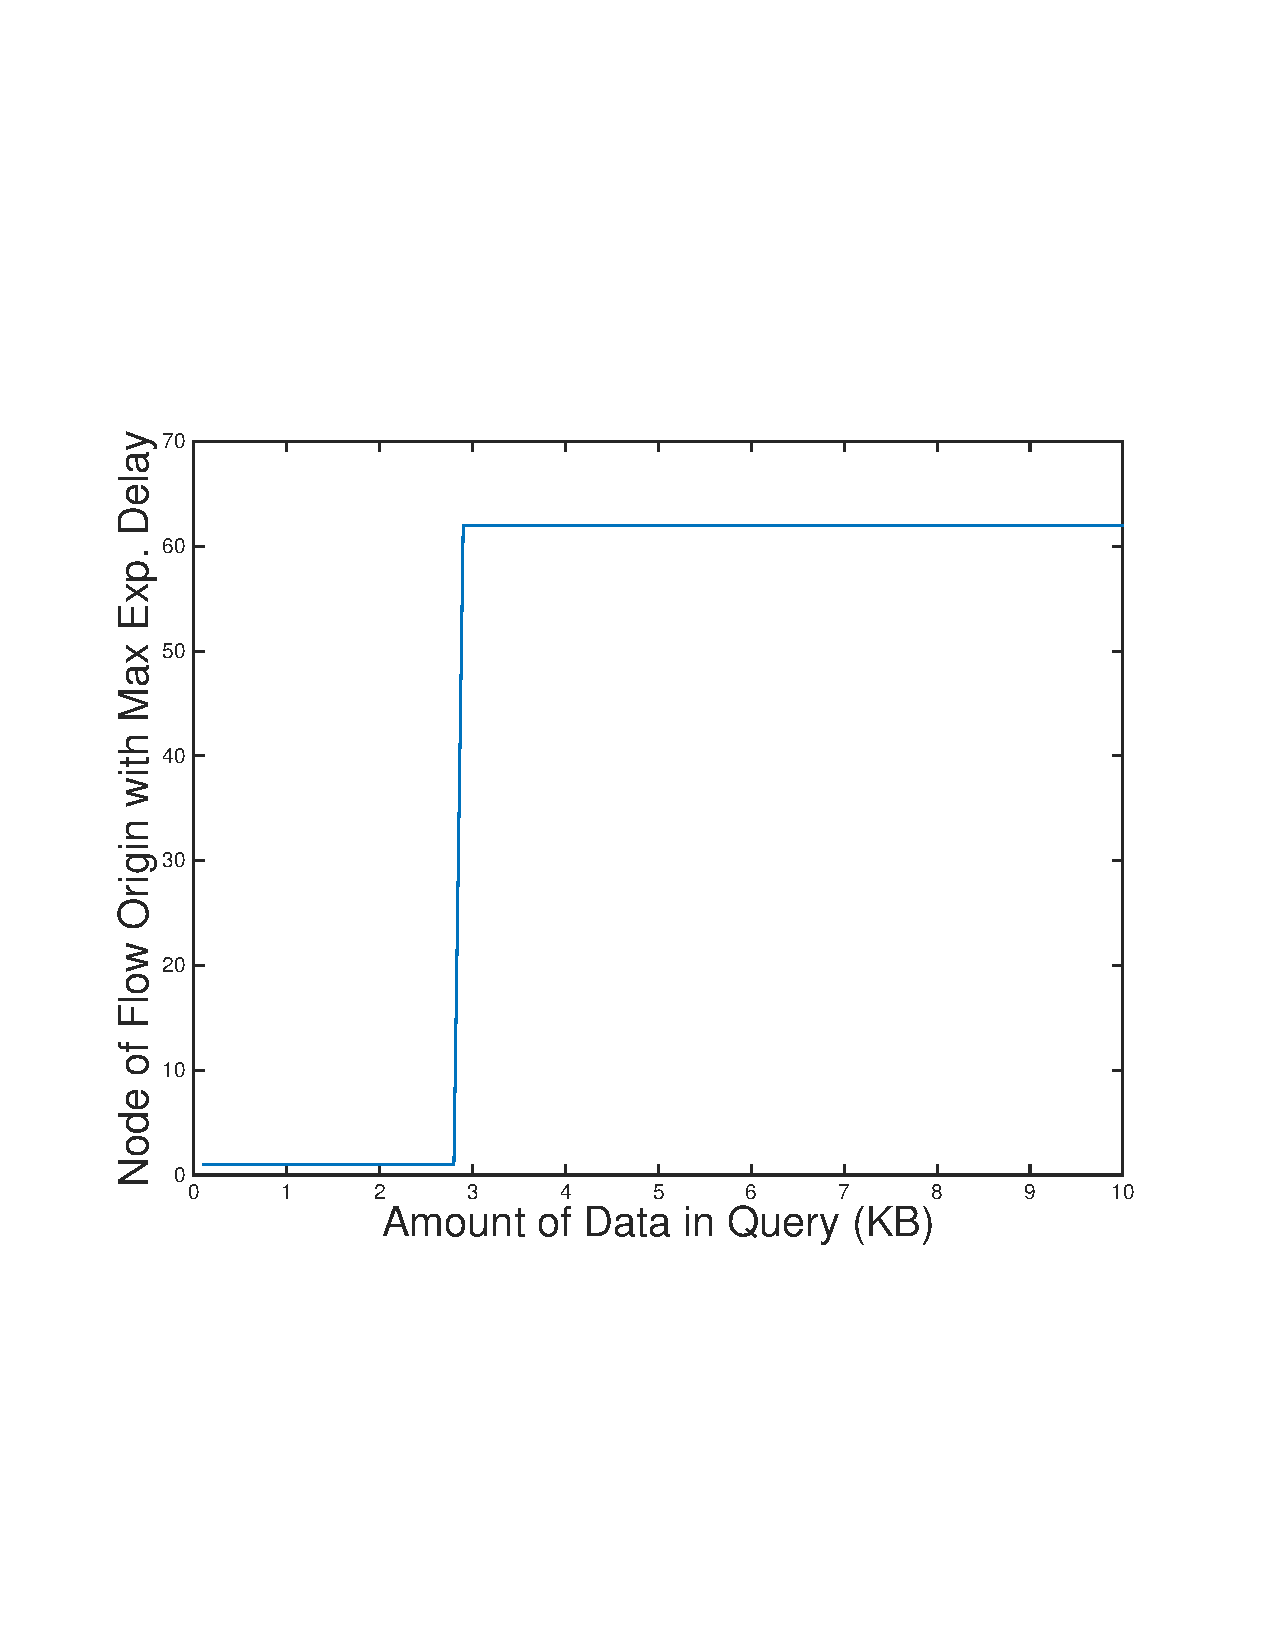
\includegraphics[scale=0.4, clip=true, trim=15mm 65mm 20mm 65mm]{figures/max_i_line_net_125.pdf}
%    \caption{The value of $i$ (origin of a flow) that causes the maximum expected delay.}
%    \label{fig:max_i_line_net}
%\end{centering}
%\end{figure}




\section{Example of Applying Framework}
\label{sec:example_applications}

We illustrate the application of Equation (\ref{eq:general_scal}) using an $N$-node TDMA network with three different topologies: clique, line, and grid, also known as a ``Manhattan grid.''  Discussion of other network control protocols and topologies are addressed in Section \ref{sec:discussion}.  We adopt a traffic model that uses Top-K queries as an example application.  We assume that all nodes have a set of collected images that are used to respond to Top-K queries.  Each node produces queries according to a Poisson process with exponential interarrival times with parameter $\lambda$, each with a target image and target QoI, $\mathbf{q} = \{C, T\}$, describing the required completeness (here, we use sum similarity) and timeliness, and sends it to another node chosen at random.  
%\footnote{This application is not necessarily intended to model a known operational scenario, only a generic example to illustrate our model in a simple manner.}  
Here, the actual size of the response fulfilling the query can be given by a distribution that incorporates the number of images required, $k_{req}$, and the size of each image.  The details of this distribution can be given from empirical observations of experiments like those in Section \ref{sec:qoi_model}.
%The queried node will respond with the required number of images, $k_{req}$, which can also be described by a distribution according to the empirical relation in Figure \ref{fig:topkSumSim}.

\subsection{Defining Traffic Factor}
\label{sec:def_tf}

The Traffic Factor will depend on the traffic pattern and routing scheme used in the network, but here we outline a general formula for modeling it with a random variable based on the traffic model described above.  
%In our formulation, we will focus on an application in which all nodes generate queries that request data of a given size from a randomly chosen destination.  We assume that these queries are generated according to a Poisson distribution with an average rate of $\lambda$.  

Let $\rho(x)$ be the number of shortest paths of all other nodes that include node $x$.  Let $\chi_{ij}$ represent the existence of a flow from node $i$ to node $j$.  We assume that $\chi_{ij}$ is equal to $1$ with probability $p_{f}$ and $0$ otherwise.  Then, the traffic factor of a node $x$, $TF_x$, is given by the sum of $\chi_{ij}$ for all $\rho(x)$ pairs $(i,j)$ in which $x$ is along the shortest path.  If $\chi_{ij}$ is i.i.d for all pairs $(i,j)$, then $TF_x$ is a Binomial random variable with $n=N$ and $p=p_{f}$.  Depending on the traffic pattern of the application(s) in the network, the conditions for using an approximation for $TF_x$ are likely to be satisfied as we show in the next section where we approximate it with a Poisson distribution.

%Assuming that $\chi_{ij}$ is i.i.d. for all pairs $(i,j)$, then, using the de Moivre-Laplace theorem, $TF_x$ can be approximated by a Normal RV with mean $\mu_{TF_x} = \rho(x) p_f$ and variance $\sigma_{TF_x}^2 = \rho(x) p_f (1-p_f)$ if the network is sufficiently large:
%\begin{equation}
%	f_{TF_x} = \mathcal{N}(\rho(x) p_f, \rho(x) p_f (1-p_f)) 
%\end{equation}
%For increased accuracy, especially in network setups that project to small maximum network sizes, continuity corrections may be useful.  Since our overall goal of estimating scalability and QoI limits allows for approximation, though, we will use this distribution as is for the $TF$.  
%When characterizing the largest contributor to delay, we need to determine the maximum expected Traffic Factor through which the flow will be forwarded.  For a given flow from $i$ to $j$, we will use $TF_{x' | i,j}$ to represent that maximum expected Traffic Factor for that flow, where $x'$ is given by  

%\begin{equation}
%\label{eq:max_tf_node}
%	x' = \argmax_{x \in \mbox{ \emph{Path from i to j}} } \mu_x % which is also = \rho(x) 
%\end{equation}

%More specifically, we can focus on just the distribution of the traffic factor with the maximum mean along the path from $i$ to $j$, $f_{TF_{x' | i,j}}$.  We will shorten the notation for this traffic factor distribution to $f_{TF_{i | j}}$.  

With a goal of determining maximum scalability and QoI-satisfiability limits, we choose to focus on the bottleneck node, $b$, which is the node that results in the largest mean $\mu_{TF_x}$ value.  While some non-uniform topologies may require some processing or calculation to determine this bottleneck node, in the topologies we explore in depth here, finding the bottleneck is intuitive.  
Next, we derive the $TF$ expression for the bottleneck node in line and grid topologies.  

\subsubsection{Line Network Traffic Factor}

First, let us look at the number of paths that go through the bottleneck node, which is the center node for a line network.  We will assume that $N$ is odd here, for simplicity of notation, but the logic is the same for even values of $N$.  Since there are $\frac{N-1}{2}$ nodes on each side the center node, the total number of paths that go through it is
\begin{equation*}
%	\rho(\frac{N}{2}) = 2(\frac{N}{2}-1)^2
%	\rho(b) = 2(\frac{N}{2}-1)^2
	\rho(b) = 2(\frac{N-1}{2})^2
\end{equation*}

Then, since there are $N$ flows and $N*(N-1)$ total paths in the network, we can approximate the probability of each path containing a flow as $p_f = \frac{1}{N-1}$.  Then, $TF_x$ will be a Binomial random variable with $n=\rho(b)$ and $p=\frac{1}{N-1}$.  Therefore, since $np$ remains fixed and $p$ approaches zero for a given network size $N$, we can use a Poisson approximation for $TF_x$ in this case, giving the following distribution:  
%We note that in other traffic patterns, e.g., when $p$ does not approach $1$ or $0$, a normal approximation may be used instead.   
\begin{equation*}
	f_{TF_b}(t) = e^{-(\frac{N-1}{2})}\frac{(\frac{N-1}{2})^{t}}{t!}
\end{equation*}
While a Poisson approximation is appropriate here, in other applications, $TF_x$ may be approximated using a Normal distribution instead, especially when $p$ does not approach zero or one for a given network size.   
%The traffic factor of the center node in a line network can then be approximated by a normal distribution as follows:
%\begin{equation*}
%	f_{TF_b} = \mathcal{N}( \frac{2(\frac{N}{2}-1)^2}{N-1}, \frac{2(\frac{N}{2}-1)^2}{N-1} \cdot ( 1 - \frac{1}{N-1} )  )
%\end{equation*}

%Next, we can determine the maximum mean of the traffic factor along the path from $i$ to $j$.  We will give the expression for values of $i < \frac{N}{2}$ here for simplicity, but note that since the network is symmetrical, it holds for all nodes.  It is easy to show that $\rho(x)$ is increasing in the domain $[1,N/2)$ with the maximum at $N/2$.  Therefore, the value of $x'$ is given by: 
%
%\begin{eqnarray*}
%	x' &=&
%		\left\{\begin{array}{ll}
%		i & \mbox{    } j < i \\
%		j & \mbox{    } i < j < \frac{N}{2} \\
%		\frac{N}{2} & \mbox{    } \frac{N}{2} \leq j \leq N \\ 
%		0 &\mbox{o.w.}
%		\end{array}\right.
%\end{eqnarray*}
%
%Therefore, we can give the expression for $f_{TF_{i | j}}$ in Equation (\ref{eq:tf_pdf_i_given_j}) where $\mu(x) = \frac{2(x-1)(N-x)}{N-1}$ and $\sigma(x) = \sqrt{\frac{2(x-1)(N-x)}{N-1} \cdot (1 - \frac{1}{N-1} )}$:
%
%\begin{eqnarray}
%	f_{TF_{i | j}} (tf) &=&
%		\left\{\begin{array}{ll}
%		\mathcal{N}( \mu(i), \sigma(i) ) & \mbox{    } j < i \\
%		\mathcal{N}( \mu(j), \sigma(j) ) & \mbox{    } i < j < \frac{N}{2} \\
%		\mathcal{N}( \mu(\frac{N}{2}), \sigma(\frac{N}{2}) ) & \mbox{    } \frac{N}{2} \leq j \leq N 
%		\end{array}\right.
%		\label{eq:tf_pdf_i_given_j}
%\end{eqnarray}

\subsubsection{Grid Network Traffic Factor}

Again, the bottleneck node, i.e., the node with the highest number of paths going through it is the center node, and we give the derivation for when $\sqrt{N}$ is odd, but the logic follows similarly for even values.  As proved in \cite{lattice_nets_cap_opt_routing}, the most optimal routing scheme for maximum capacity is ``Row-First, Column-Second" routing, so we assume paths follow this approach.  Again, we adopt a traffic pattern in which each node is the source of exactly one flow and that the destination is uniformly chosen from all other $N-1$ nodes.  
%Node $i$, then, has a $\frac{1}{N-2}$ chance of choosing each non-center node.  
For each source node, we can determine the number of destinations that route through the center.  We separate nodes into two categories for this counting.

\begin{figure}
\begin{centering}
    \includegraphics[scale=0.39]{figures/TF_proof_fig_color.pdf}
    \caption{Sources and destinations used in proving TF for grid networks}
    \label{fig:TF_proof_fig}
\end{centering}
\end{figure}

First, we consider the nodes circled in set $A$ in Figure \ref{fig:TF_proof_fig}, of which there are $\sqrt{N} \cdot \frac{\sqrt{N}-1}{2}$.  Through manual inspection, one can deduce that the only destination nodes in the figure that result in a path that is relayed by the center node are the two bottom nodes in the center column in the figure, marked with blue.  
%The probability of a node in set $A$ choosing one of these destinations is $P_{A} = \frac{\frac{\sqrt{N}-1}{2}}{N-2}$.
%Now, we can count the total number of nodes for which this probability holds.  From the figure, we can quantify the number of circled nodes, but we must also consider the reverse, i.e. imagine the figure rotated vertically, so the total number of nodes falling into set $A$, including the mirror of those circled in the figure, is $N_A = \sqrt{N} \cdot (\sqrt{N}-1)$.
There are $\frac{\sqrt{N}-1}{2}$ of these destination nodes for the nodes in set $A$, so the total number of paths from the nodes in set $A$ is $\sqrt{N} \cdot (\frac{\sqrt{N}-1}{2})^2$.  Now, if we also consider the reverse, i.e. imagine the figure rotated vertically, then we can give the total number of paths from nodes not in the same row as the center node as $2 \cdot \sqrt{N} \cdot (\frac{\sqrt{N}-1}{2})^2$.
%Now, we can count the total number of nodes for which this probability holds.  From the figure, we can quantify the number of circled nodes, but we must also consider the reverse, i.e. imagine the figure rotated vertically, so the total number of nodes falling into set $A$, including the mirror of those circled in the figure, is $N_A = \sqrt{N} \cdot (\sqrt{N}-1)$.
%Then, the contribution to the TF by nodes in set $A$ is simply the product of $P_A$ and $N_A$:
%\begin{equation}
%	E[TF_{A}] = \frac{\frac{\sqrt{N}-1}{2}}{N-2}  \cdot  \sqrt{N} \cdot (\sqrt{N}-1)
%\end{equation}

Next, we consider the nodes in the same row as the center node, which we call set $B$.  
Here, all destinations on the ``opposite" side of the center as well as those in the same column of the center require being routed through the center node when originating from any nodes in set $B$.  Just as above, we can count the number of paths from the nodes in set $B$ that route through the center and double it to count the reverse.  The resulting number of paths is $2 \cdot (\sqrt{N} \cdot \frac{\sqrt{N}+1}{2}-1) \cdot (\frac{\sqrt{N}-1}{2})$.
%Just as above, we can relate the probability of choosing one of these destinations as $P_{B} = \frac{\frac{\sqrt{N}+1}{2} \cdot \sqrt{N} - 1}{N-2}$ and $N_{B} = \sqrt{N}$, so the expected contribution to TF from set $B$ is
%\begin{equation}
%	E[TF_{B}] = \frac{\frac{\sqrt{N}+1}{2} \cdot \sqrt{N} - 1}{N-2} \cdot 2 \cdot (\frac{\sqrt{N}-1}{2})
%\end{equation}
%
%Since sets $A$ and $B$ account for all non-center nodes in the network, the overall expected traffic factor is just the sum of $E[TF_A]$ and $E[TF_B]$, which simplifies to
%\begin{equation}
%	E[TF] = \frac{\sqrt{N}(N - 2) + 1}{N-2}
%\end{equation}
%which is effectively $\sqrt{N}$ for large $N$.

Adding together these paths and simplifying gives us the following expression for the total number of paths that go through the center node: 
\begin{equation}
%	\rho(\frac{N}{2}) = \sqrt{N} \cdot (N-2) + 1
	\rho(b) = \sqrt{N} \cdot (N-2) + 1
\end{equation}
Just as with line networks, the probability of each path containing a flow is $p_f = \frac{1}{N-1}$, so the traffic factor for the center node of a grid network is approximated with a Poisson distribution:
\begin{equation*}
%	f_{TF_b} = \mathcal{N}( \frac{\sqrt{N} \cdot (N-2) + 1}{N-1}, \frac{\sqrt{N} \cdot (N-2) + 1}{N-1} \cdot ( 1 - \frac{1}{N-1} )  )
	f_{TF_b}(t) = e^{-(\frac{\sqrt{N}\cdot(N-2)+1}{N-1})}\frac{(\frac{\sqrt{N}\cdot(N-2)+1}{N-1})^{t}}{t!}
\end{equation*}
which can be approximated by the following for large values of $N$.  
\begin{equation*}
%	f_{TF_b} = \mathcal{N}( \sqrt{N}, \sqrt{N} \cdot ( 1 - \frac{1}{N-1} )  )
	f_{TF_b}(t) = e^{-(\sqrt{N})}\frac{(\sqrt{N})^{t}}{t!}
\end{equation*}

%Since our goal is to determine the point at which an average flow is no longer sustainable, we derive expressions for $TF$, $CF$, and $DF$ for the network.  In the case of $TF$, we use the value for the node with the largest expected $TF_i$ since flows that are routed through this node are expected to experience that largest delay and are likely to be the first that fail to meet their timeliness requirements.  Values for this example are shown in Table \ref{table:rf_ff_sf_values}. A derivation of $TF$ for a grid network is included in Appendix \ref{sec:grid_tf_proof}.  Details about deriving the other values are explained in \cite{symptotics_journal}.  The equations in Table \ref{table:scal_eqs} can be used to determine QoI and network size limitations.


\subsection{Scalability Equations}

Once an expression for the Traffic Factor ($TF$) is derived, we can use it along with expressions for the Channel Factor ($CF$), Delay Factor ($DF$), and Path Length ($PL$) for the network to create specific instances of Equation (\ref{eq:general_scal}) that estimate the scalability and QoI-satisfiability limits of the particular network of interest.  Since our goal is to determine the point at which the system is unable to support the offered traffic load within the timeliness constraints, we use maximum values for these factors where applicable, specifically $TF_{max}$ and $PL_{max}$.  

\begin{table*}[]
\centering
\begin{tabular}{l|l|l|l|l|l|}
\cline{2-6}
%                            					 & \boldmath{$CF$}  			& \boldmath{$TF_{\mu}$}   			& \boldmath{$TF_{\sigma}$}										& \boldmath{$DF$}			& \boldmath{$PL_{max}$}	\\ \hline
                            					 & \boldmath{$CF$}  			& \boldmath{$\mu_{TF}$}   			& \boldmath{$\sigma_{TF}$}										& \boldmath{$DF$}			& \boldmath{$PL_{max}$}	\\ \hline
\multicolumn{1}{|l|}{\textbf{Clique}} 	& $N-1$ 						& $1$                            				& $1$                            												& $1$  						& $1$ 					\\ \hline
\multicolumn{1}{|l|}{\textbf{Line}}   	& $3$   							& $\frac{N-1}{2}$ 					& $\sqrt{\frac{N-1}{2}}$ 		& $1.5$						& $N-1$				\\ \hline
\multicolumn{1}{|l|}{\textbf{Grid}}   	& $5$   							& $\sqrt{N}$                       			&$N^{\frac{1}{4}}$							&  $2.5$					& $2 \cdot \sqrt{N}$   	\\ \hline
\end{tabular}
\caption{CF, TF, DF, and PL values for example topologies}
\label{table:rf_ff_sf_values}
\end{table*}

\begin{table*}[]
\centering
\begin{tabular}{l|l|}
\cline{2-2}
                             & \multicolumn{1}{c|}{{\bf Equation}} \\ \hline
\multicolumn{1}{|l|}{\textbf{Clique}} & \multicolumn{1}{c|}{$W \cdot T - I_S \cdot k_{req} \cdot (N-1) \geq 0$}            \\ \hline
\multicolumn{1}{|l|}{\textbf{Line}}   & \multicolumn{1}{c|}{$W \cdot T - 3 \cdot I_S \cdot k_{req} \cdot (\frac{N-1}{2} + \eta \cdot \sqrt{\frac{N-1}{2}}) - 1.5 \cdot P_S \cdot (N-1) \geq 0$}       \\ \hline
\multicolumn{1}{|l|}{\textbf{Grid}}   & \multicolumn{1}{c|}{$W \cdot T - 5 \cdot I_S \cdot k_{req} \cdot (\sqrt{N} + \eta\cdot N^{\frac{1}{4}}) - 2.5 \cdot P_S \cdot (2 \cdot \sqrt{N} - 1) \geq 0$}      \\ \hline
\end{tabular}
\caption{Scalability equations}
\label{table:scal_eqs}
\end{table*}

The $PL_{max}$ is usually quickly determined by an examination of the topology, such as $PL_{max} = N-1$ for a line network and $PL_{max} = 2 \cdot \sqrt{N}$ for a grid network.  To get a good estimate of $TF_{max}$, we can simply utilize the mean and standard deviation of the distribution derived above to create the following: $TF_{max} = \mu_{TF} + \eta \cdot \sigma_{TF}$ where $\eta$ is a factor that can adjust how conservative the estimates should be.  This notion of $\eta$ is analogous to the z-score of a standard normal distribution, and is applicable here since $TF_x$ approaches a Normal distribution as the network size, $N$, grows.  As an example, we use $\eta = 3.5$ in the validation results below, which captures approximately $99.7\%$ of the maximum of the $TF$ distribution.  

Table \ref{table:rf_ff_sf_values} shows expressions for clique, line, and grid networks as derived above and in \cite{symptotics_journal}.  Then, substituting the factors into equation \ref{eq:general_scal}, we achieve the scalability equations for each topology in Table \ref{table:scal_eqs}.  


To find the limitation of a particular parameter or QoI component, the scalability equation can be solved for the variable of interest.  Then all known values can be substituted to get the limit of the variable of interest.  For example, given a network size and completeness requirement, we can determine a clique network's minimum sustainable timeliness with the equation $T  \geq \frac{I_S \cdot k_{req} \cdot (N-1)}{W}$, where $k_{req}$ is given by the completeness function $Q(C)$.  In practice, solutions for these equations will most likely need to be made numerically, but doing so is rather straightforward using any number of commonly available tools.  As we will show in Section \ref{sec:network_design}, these equations can also be easily used to determine the impact of other network parameters on this timeliness limit. 

\subsection{Minimum Timeliness/Maximum Query Rate}

Solving the Scalability equations for $T$ reveals the minimum satisfiable timeliness value for which all queries are expected to complete within the deadline constraint, which we will call $T_{min}$.  Consequently, this minimum satisfiable timeliness value also correlates to the maximum traffic rate that can be served by the network, $\lambda_{max} = \frac{1}{T_{min}}$.  If the average rate of queries, $\lambda$, is greater than $\frac{1}{T_{min}}$, then the traffic will exceed the network capacity and the number of active queries in the system will grow without bound, causing packets to be dropped and/or delays to grow without bound.  Therefore, the maximum query rate is $\lambda_{max} = \frac{1}{T_{min}}$, and, consequently, the minimum timeliness for which \emph{all} flows can be expected to complete before the deadline is $T_{min}$.

%To determine maximum expected delay, $d_{max}$, of a flow in the network, which occurs at the delay $d$ at which $F_{D}$ reaches its maximum value of $1$.  If the average rate of queries, $\lambda$, is greater than $\frac{1}{d_{max}}$, then the traffic will exceed the network capacity and the number of active queries in the system will grow without bound, causing packets to be dropped and/or delays to grow without bound.  Therefore, the maximum query rate is $\lambda_{max} = \frac{1}{d_{max}}$, and, consequently, the minimum timeliness for which \emph{all} flows can be expected to complete before the deadline is $d_{max}$.

In some applications, having a certain amount of queries not complete by the timeliness requirement may be acceptable.  As we show in Section \ref{sec:delay_char}, we can develop a more detailed characterization of the delay equation than the Scalability Equations here for these applications. 
%In some applications, having a certain amount of queries not complete by the timeliness requirement may be acceptable.  In these situations, more useful information can be extracted from the delay distribution in Equation (\ref{eq:full_delay_cdf}).  Specifically, this delay distribution can be interpreted as the expected percentage of queries that will finish within the timeliness constraint if the timeliness constraint was $d$.  As we will show in Section \ref{sec:example_applications}, this relationship follows a Normal distribution CDF.

\subsection{Validation of Scalability Equations}
\label{sec:validation}

%\setcounter{MYtempeqncnt}{\value{equation}}
\begin{figure*}[!t]
\setcounter{equation}{9}
\begin{equation}
\label{eq:full_delay_cdf}
	F_D(d) = \frac{1}{N} \cdot \sum\limits_{i = 1}^N \sum\limits_{j \neq i} \sum\limits_{tf=1}^{tf_{max}}  F_{P_N}( \frac{d - C_2 \cdot PL(i,j)}{C_1 \cdot p_N} ) \cdot f_{TF_{i | j}}( tf ) \cdot p(j)
\end{equation}
\end{figure*}
\setcounter{equation}{5}
%\setcounter{equation}{\value{MYtempeqncnt}}

\begin{figure}[]
\centering
       \subfigure[Line Network, $I_S = 18 KB$]{
        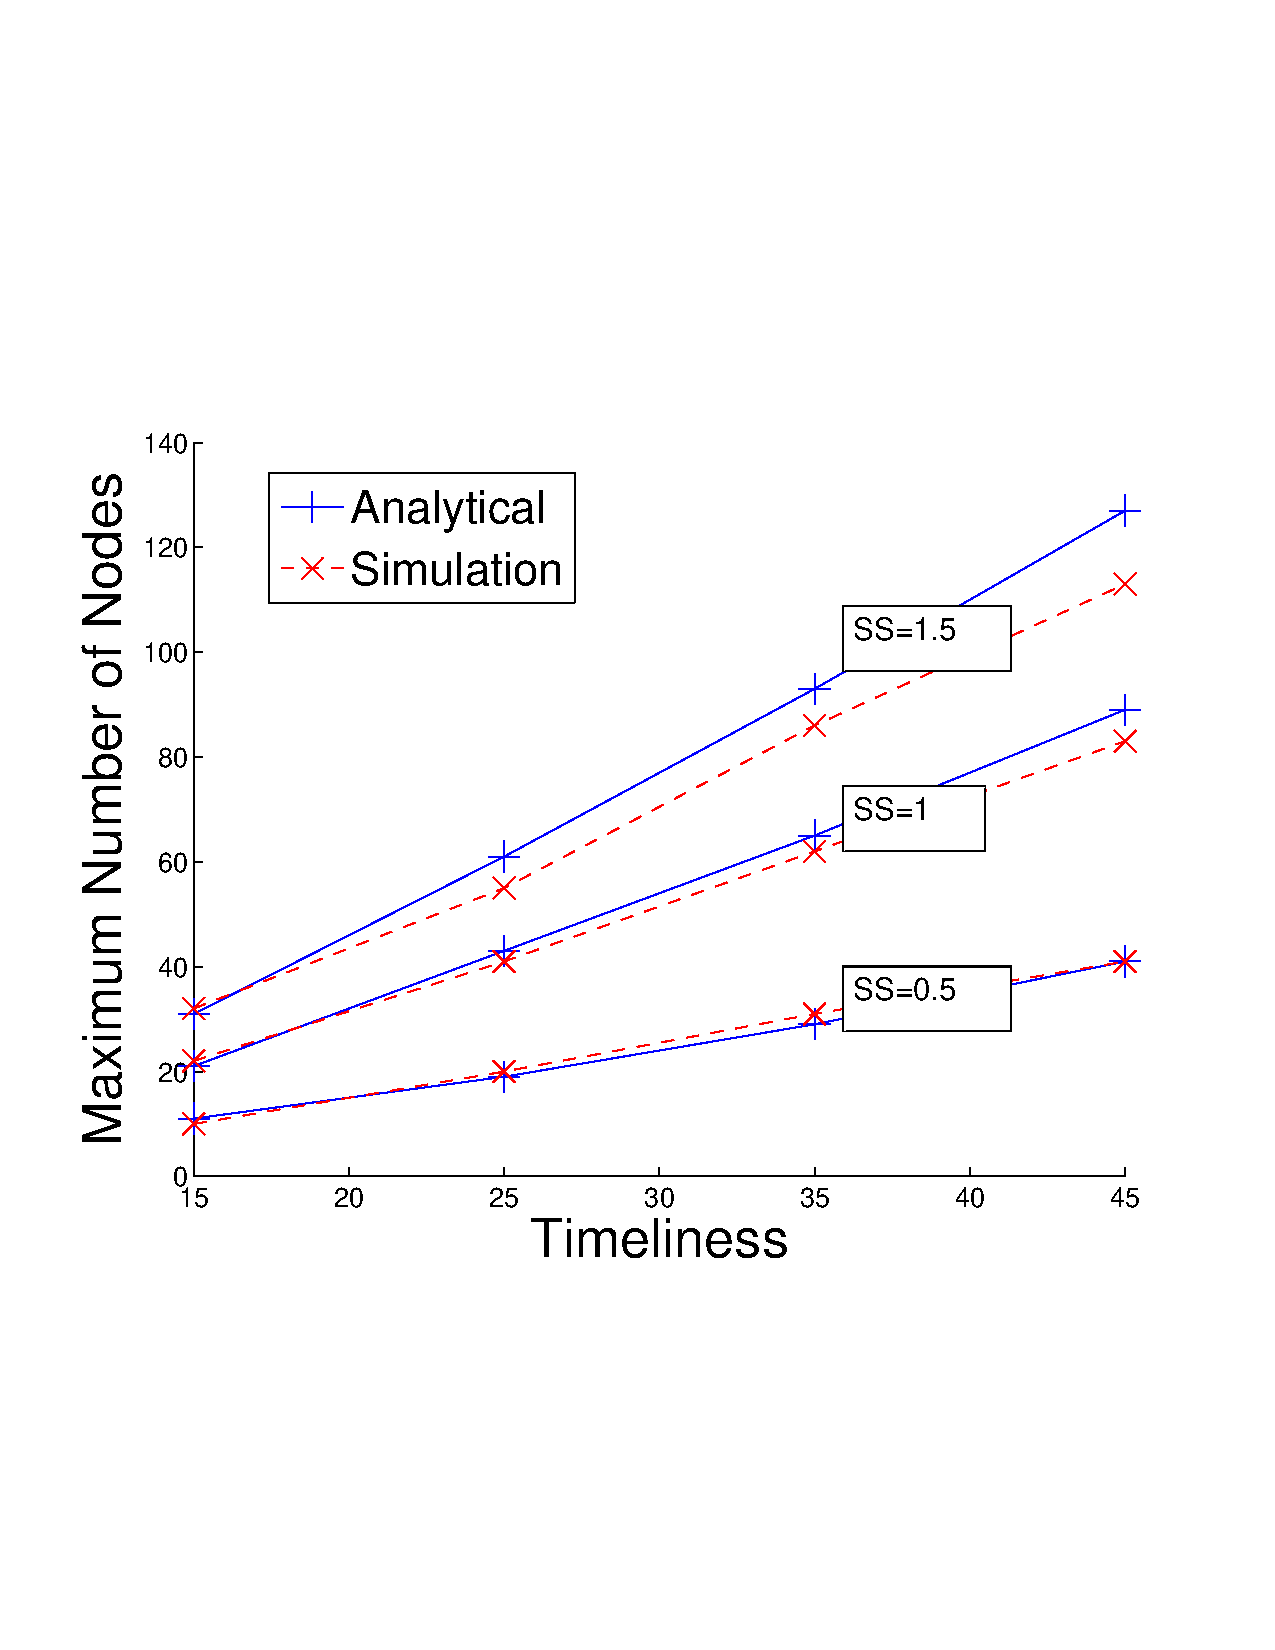
\includegraphics[scale=0.40, clip=true, trim=12mm 65mm 20mm 65mm]{figures/scal_sim_results/line_scal_anal_vs_sim_color.pdf}
%        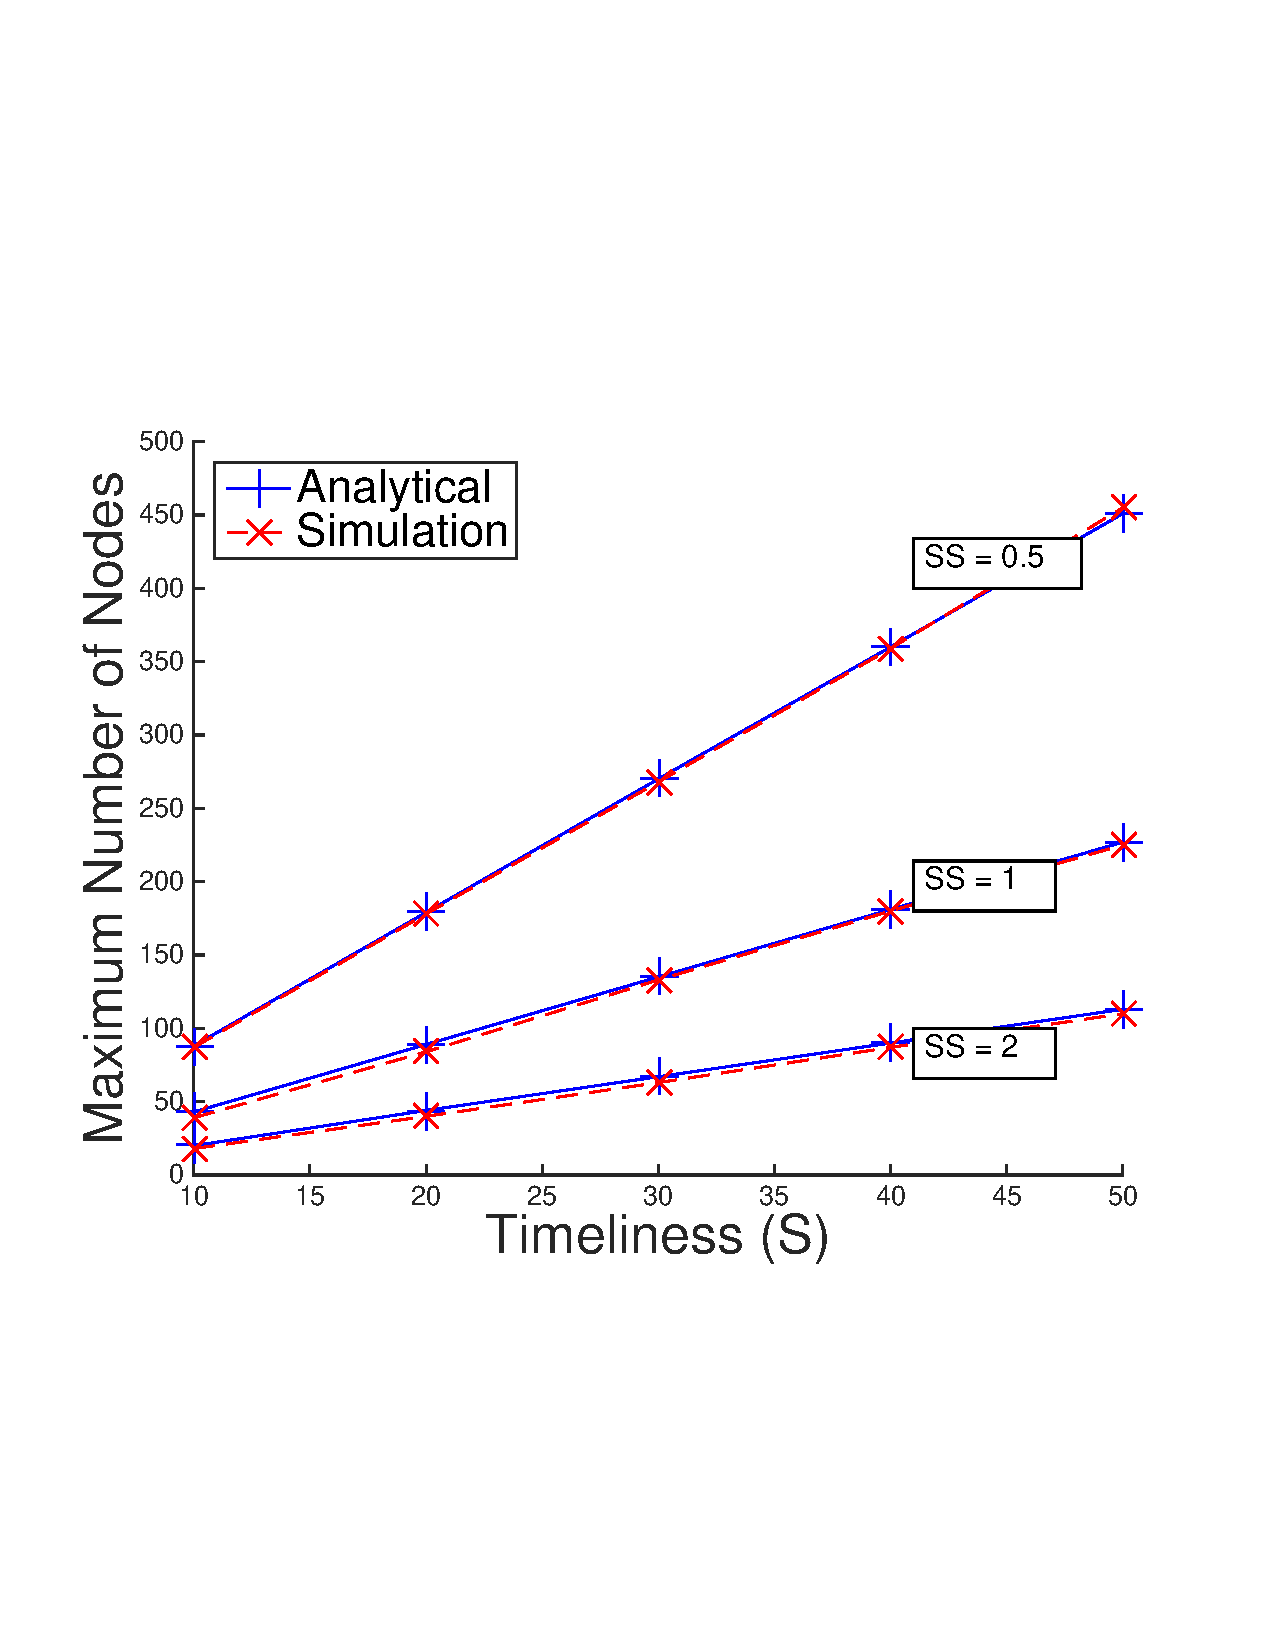
\includegraphics[scale=0.40, clip=true, trim=12mm 65mm 20mm 65mm]{figures/scal_sim_results/color_2d/line_uni_2d_qoi_vs_non_color_multiple.pdf}
        \label{fig:scal_vs_qoi_line}
        }
    \subfigure[Grid Network, $I_S = 48 KB$]{
%        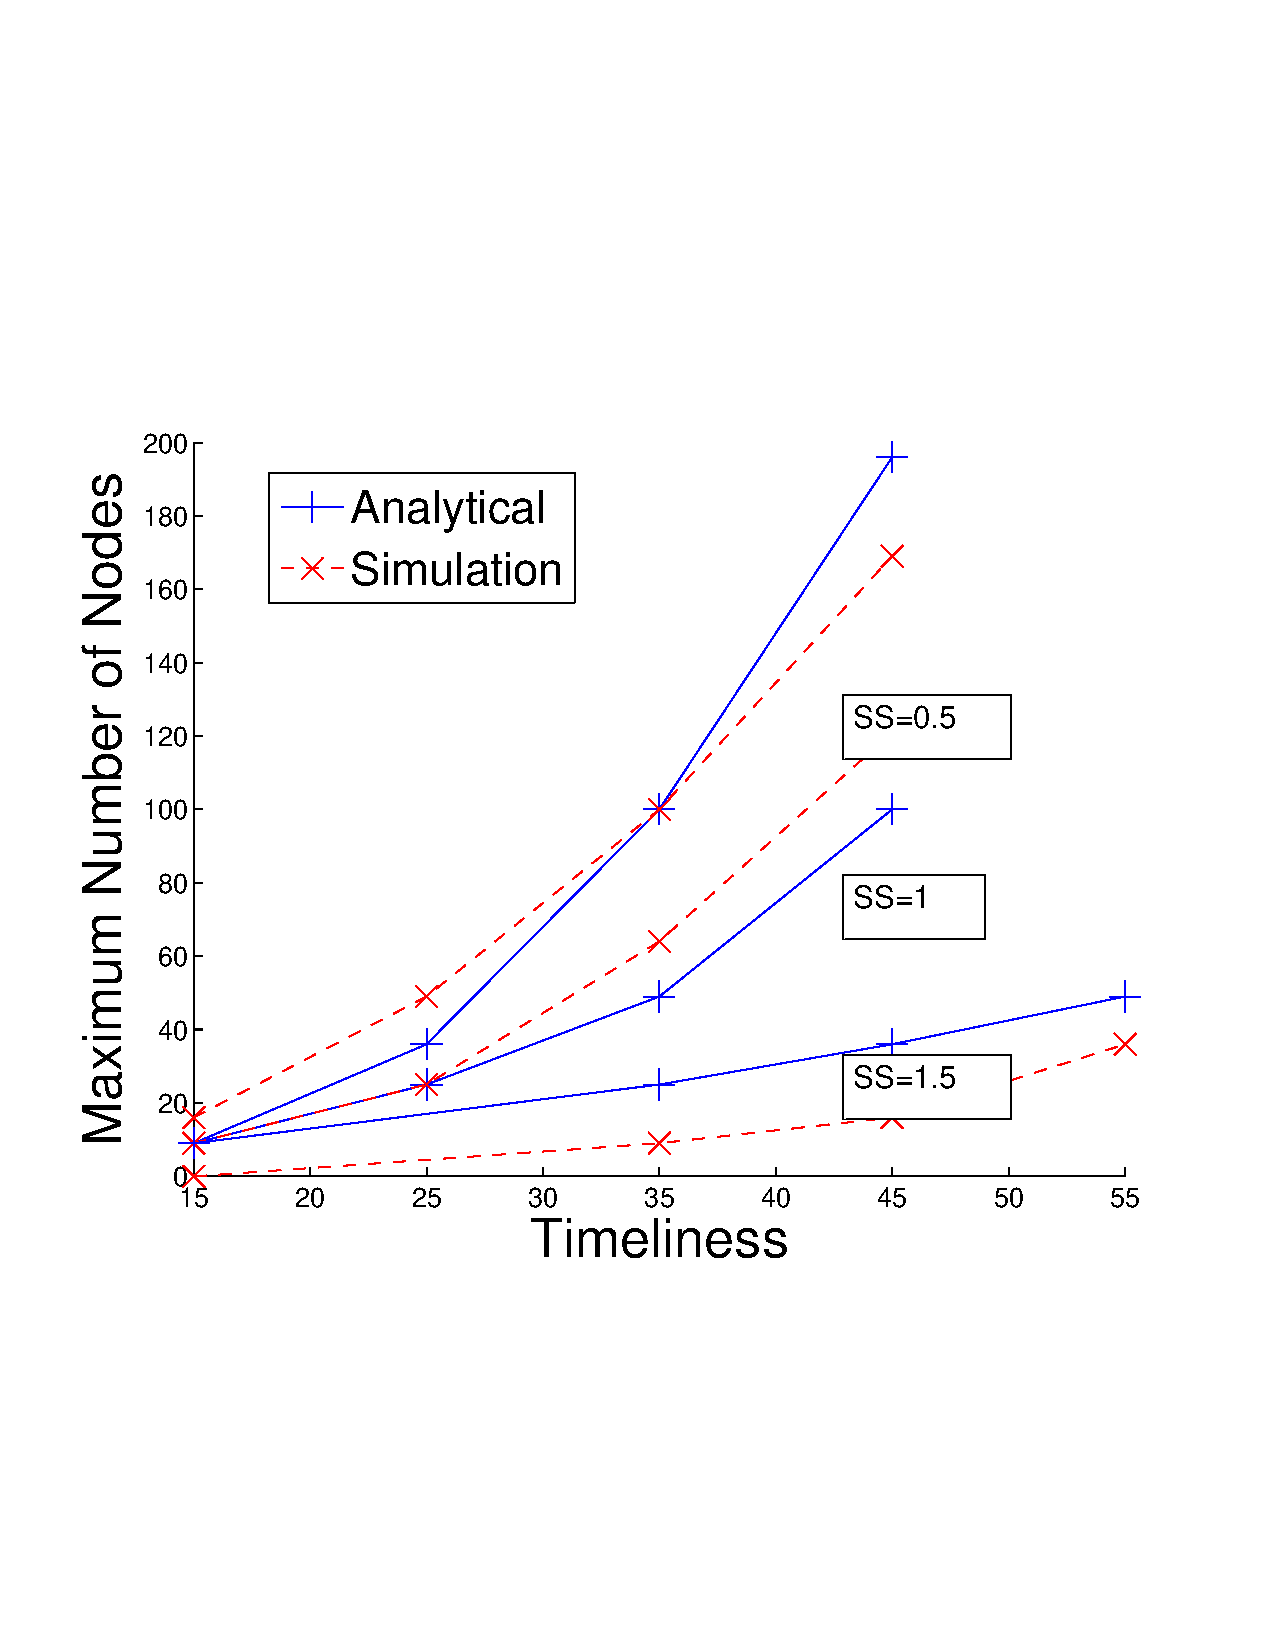
\includegraphics[scale=0.40, clip=true, trim=12mm 65mm 20mm 65mm]{figures/scal_sim_results/grid_scal_anal_vs_sim_color.pdf}
        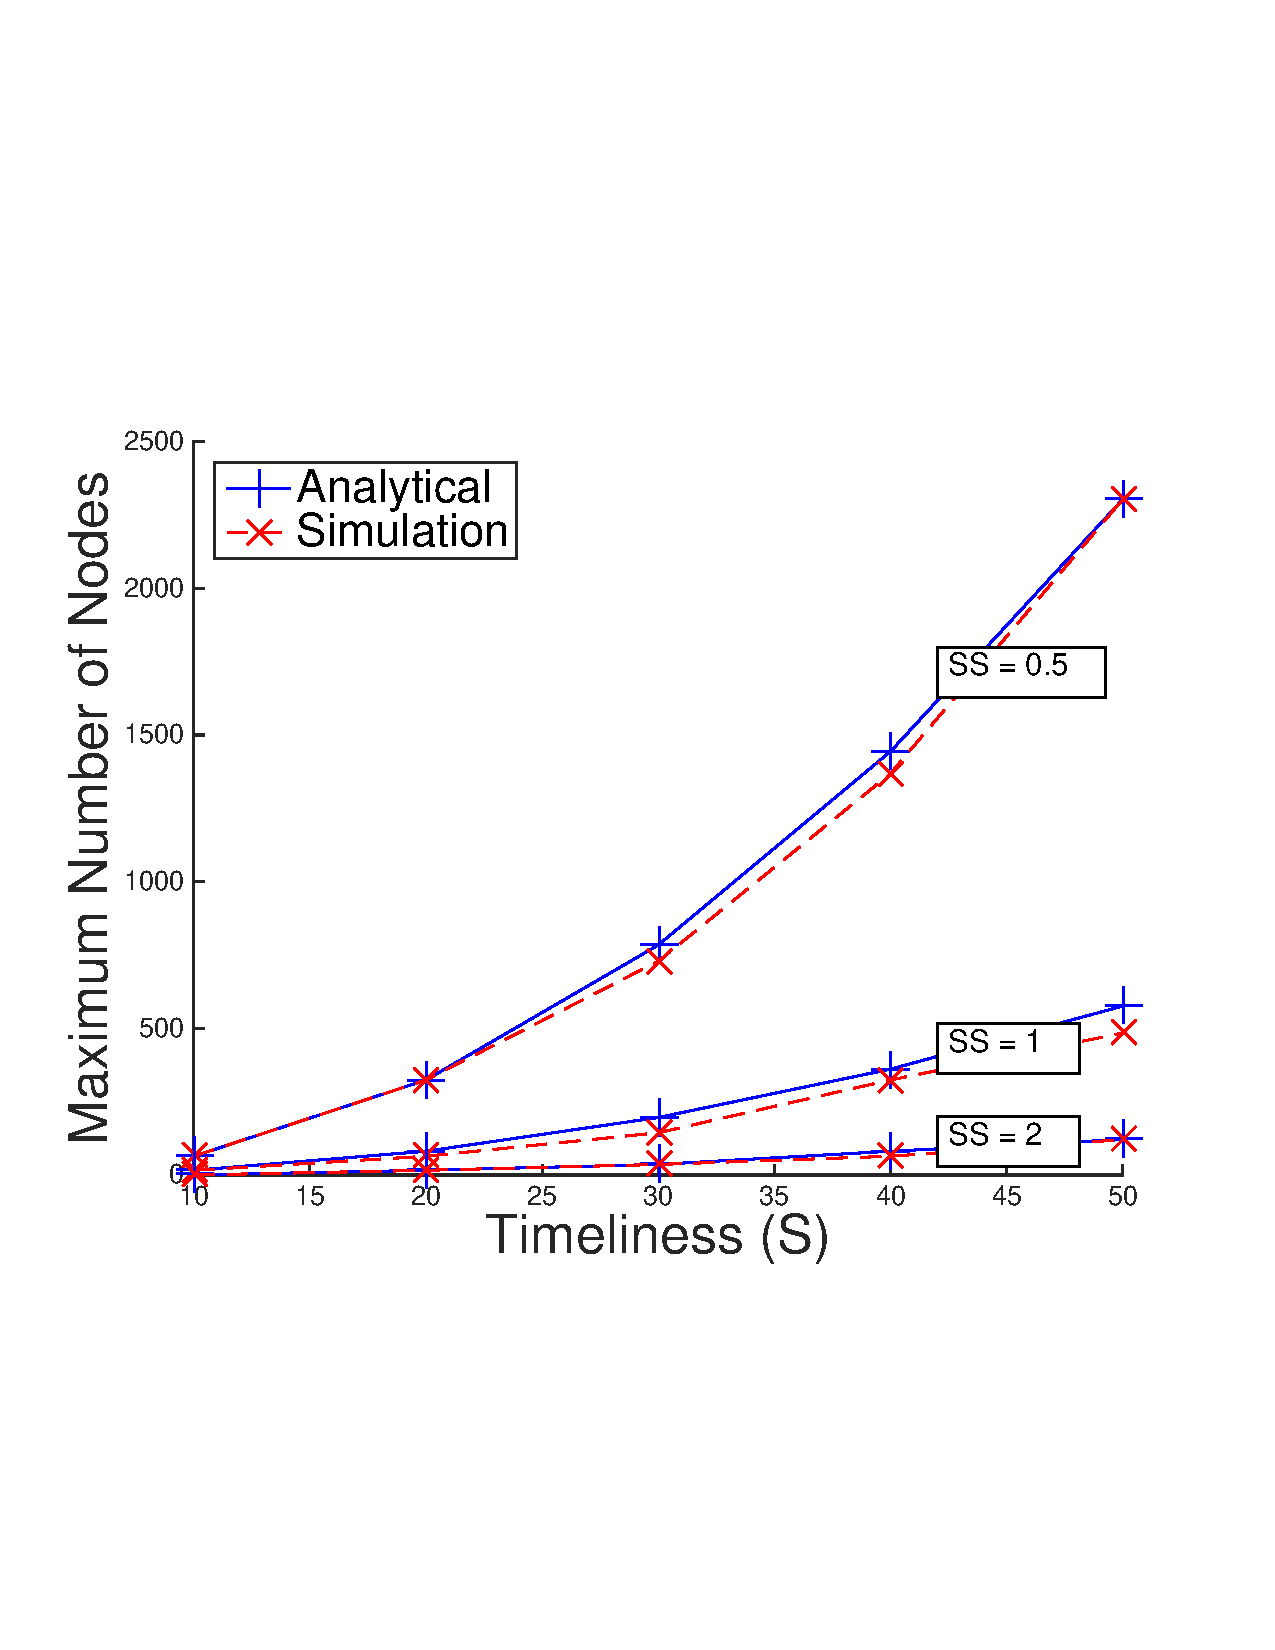
\includegraphics[scale=0.40, clip=true, trim=12mm 65mm 20mm 65mm]{figures/scal_sim_results/color_2d/grid_uni_2d_qoi_vs_non_color_multiple.pdf}
        \label{fig:scal_vs_qoi_grid}
        }
   \caption{Empirical results match analytical results closely for all tests.}
   \label{fig:scal_vs_qoi}
\end{figure}

To show how effective estimates using this framework can be, we simulated the network topologies and traffic described above in Section \ref{sec:example_applications} in the ns3 network simulator, comparing empirical results to those generated analytically with this framework, labeled \emph{Analytical}.  
%Due to space concerns, we only show a subset of results in Figure \ref{fig:scal_vs_qoi} to provide evidence of the effectiveness of the methodology.  All results generated, however, exhibit very similar trends of proximity between empirical and the analytical values.
We use a channel rate of $W= 2 Mbps$, packet sizes of $P_s = 1500$ bytes, and image sizes of $18$ and $48$ Kbytes.  As above, the correlation between Sum Similarity and $k_{req}$ is taken from the actual observed relation in Figure \ref{fig:topkSumSim}.  All values of parameters ($SS$, $T$, $I_S$, etc.) were chosen to test a variety of network sizes and QoI requirements while remaining within realistic network sizes, both with respect to real-world deployments and simulations with feasible run-times.



%\section{Conclusion}
\label{sec:conclusion}

% Problem
This work provides several contributions to the field of QoI-aware wireless networks.  
%In this work, we examined network capacity and design with explicit Quality of Information consideration from a practical standpoint.
% Solution
% method and results
First, we motivated the use of completeness and timeliness as QoI attributes, providing an example application and several different ways to measure completeness.  
%We support this motivation with results from running these image selection algorithms on a real data set.
Next, we developed a framework that can be used to predict QoI and network size limits for a specific network as well as predict expected probabilities of satisfying timeliness constraints beyond the point in which all queries are satisfied.  We validated these models' accuracy by comparing analytical results with simulations performed in the ns3 network simulator in both cases.
% Take away : Lesson
Examples of the impact of different network parameters were shown, providing concrete examples of the framework's usefulness in real-world applications.  In addition, the concept of scalably feasible QoI regions was introduced.
% Future work
For future work, we plan to make generalizations of factors that will allow for easy application of this framework to any non-regular network topology and expand this framework to include consideration of more complex network control actions, such as caching and/or data compression or fusion, which are all of interest in QoI-aware networking.




%\appendix
%\input{sections/random_explanation}
% conference papers do not normally have an appendix


% use section* for acknowledgement
%\section*{Acknowledgment}


%The authors would like to thank...


% trigger a \newpage just before the given reference
% number - used to balance the columns on the last page
% adjust value as needed - may need to be readjusted if
% the document is modified later
%\IEEEtriggeratref{8}
% The "triggered" command can be changed if desired:
%\IEEEtriggercmd{\enlargethispage{-5in}}

% references section

% can use a bibliography generated by BibTeX as a .bbl file
% BibTeX documentation can be easily obtained at:
% http://www.ctan.org/tex-archive/biblio/bibtex/contrib/doc/
% The IEEEtran BibTeX style support page is at:
% http://www.michaelshell.org/tex/ieeetran/bibtex/
%\bibliographystyle{IEEEtran}
% argument is your BibTeX string definitions and bibliography database(s)
%\bibliography{IEEEabrv,../bib/paper}
%
% <OR> manually copy in the resultant .bbl file
% set second argument of \begin to the number of references
% (used to reserve space for the reference number labels box)
%\begin{thebibliography}{1}


\bibliographystyle{unsrt}

\bibliography{references}

%\bibitem{IEEEhowto:kopka}
%H.~Kopka and P.~W. Daly, \emph{A Guide to \LaTeX}, 3rd~ed.\hskip 1em plus
%  0.5em minus 0.4em\relax Harlow, England: Addison-Wesley, 1999.

%\end{thebibliography}




% that's all folks
\end{document}


